\documentclass{article}
\usepackage{graphicx} % Required for inserting images
\usepackage{fancyhdr}
\usepackage[utf8]{inputenc}
\usepackage{hyperref}
\usepackage{float}
\usepackage{pdfpages}
\usepackage{url}
\usepackage[T1]{fontenc}
\usepackage[francais]{babel}
\usepackage{tabularx}
\usepackage{indentfirst}
\usepackage{mdframed}
\usepackage{amsmath}
\usepackage{hyperref}
\usepackage{pgfgantt}
\usepackage{geometry}
\geometry{margin=1in}


\setlength{\headheight}{30pt}
\setlength{\headsep}{45pt}

\lhead{
\includegraphics[height=2cm]{Logo UT.png}}
\rhead{
\includegraphics[height=2cm]{Logo GEII.png}}

\begin{document}
\pagestyle{fancy}
\renewcommand{\footrulewidth}{0.4pt}
\lfoot{Théo Ly - Sagesse Fontarel} 
\rfoot{Cahier de laboratoire}

\begin{titlepage}
    \newcommand{\HRule}{\rule{\linewidth}{0.5mm}}
    \center
    \textsc{\LARGE} \\[1cm]
    \HRule \\[0.4cm]
    { \huge \bfseries Cahier de laboratoire – SAÉ Électronique S3 : Conception d’un ECG \\[0.3cm] }
    \HRule \\[0.5cm]
    Théo LY - Sagesse Fontarel
    \\[1cm]
    IUT Toulouse 2025-2026
     \\ [1cm]
     \thispagestyle{empty}
\end{titlepage}


\newpage
\setcounter{page}{1}
\tableofcontents
\newpage

%----------------------------------
% INTRODUCTION
%----------------------------------
\subsection{Introduction}

Dans le cadre de la SAÉ Électronique du semestre 3 à l’IUT de Toulouse, nous avons pour objectif de concevoir, vérifier et valider une carte électronique capable de mesurer et de conditionner un signal électrocardiographique (ECG). Ce projet s’inscrit dans un contexte professionnel où une entreprise souhaite développer un dispositif de mesure fiable et sûr, destiné à l’observation de l’activité cardiaque.

L’électrocardiogramme permet de visualiser les signaux électriques produits par le cœur à travers des électrodes placées sur le corps du patient. Ces signaux, d’amplitude très faible (quelques millivolts), doivent être amplifiés et filtrés avant de pouvoir être analysés ou numérisés. La carte réalisée doit ainsi assurer plusieurs fonctions : amplification, filtrage des bruits parasites (notamment le 50 Hz), suppression de la composante continue, et adaptation du signal pour une carte d’acquisition Nucleo. Un indicateur lumineux doit également permettre de visualiser le pouls du patient.

Le projet est réalisé en équipe, chaque binôme étant chargé de concevoir et de tester une ou plusieurs fonctions du système complet. L’ensemble des fonctions sera ensuite intégré afin d’obtenir un prototype opérationnel répondant aux exigences du cahier des charges.  
Le présent cahier de laboratoire retrace l’ensemble des étapes de conception, de simulation, de réalisation et de test des fonctions qui nous ont été attribuées.



%----------------------------------
% 1. LE PLANNING
%----------------------------------
\subsection{Le planning}

Le planning ci-dessous présente l'organisation prévisionnelle du travail pour la SAÉ, incluant les étapes de conception, simulation, soudure, et tests.\\ 
\\ 
\\
\begin{tabularx}{\textwidth}{|c|X|}
\hline
\textbf{Semaine} & \textbf{Activités principales} \\
\hline
\textbf{Semaine 1} & 
\begin{itemize}
  \item Formation des équipes et création des espaces Teams.
  \item Compréhension du principe de l’ECG (vidéos et documents).
  \item Analyse fonctionnelle et remplissage du schéma fonctionnel.
  \item Conception des fonctions « alimentation » et « tension de référence ».
  \item Préparation pour la 2\textsuperscript{e} séance (répartition des fonctions, validation enseignants).
\end{itemize} \\
\hline
\textbf{Semaine 2} &
\begin{itemize}
  \item Vérification et maintenance de la carte d’alimentation.
  \item Conception et dimensionnement de la première fonction attribuée.
  \item Réalisation sur protoboard et simulation.
  \item Tests unitaires et premiers tests d’intégration partielle.
  \item Rédaction du cahier de laboratoire.
\end{itemize} \\
\hline
\textbf{Semaine 3} &
\begin{itemize}
  \item Finalisation des fonctions pour un test d’intégration complet.
  \item Test avec filtre réjecteur et retour à la cheville.
  \item Conception et tests des nouvelles fonctions.
  \item Avancement du cahier de laboratoire et des fiches portfolio.
\end{itemize} \\
\hline
\end{tabularx}

\newpage

---

%----------------------------------
% 2. ANALYSE FONCTIONNELLE
%----------------------------------
\subsection{Analyse fonctionnelle du projet}

L’analyse fonctionnelle a permis d’identifier les principales fonctions du système ECG et de déterminer les gains associés à chaque étage :

\begin{itemize}
    \item Amplificateur de différence : \(G = 12\)
    \item Filtre passe-haut à gain variable : \(G = 10 \rightarrow 30\)
    \item Filtre réjecteur : \(G = 2\)
    \item Filtre passe-bas : \(G = 2\)
\end{itemize}

Le gain global du système est donc compris entre 500 et 1500, conformément au cahier des charges.

\begin{figure}[h!]
    \centering
    
\includegraphics[width=0.9\textwidth]{20251024_080742.jpg}
    \caption{Schéma-bloc fonctionnel du système ECG.}
\end{figure}

\newpage



\section{Étude des fonctions}


\subsection{Fonction d’alimentation}

\subsubsection{Introduction à la fonction}

La première étape du projet consiste à vérifier et valider la fonction d’alimentation, indispensable au bon fonctionnement du système complet. Cette carte a pour rôle de fournir les tensions continues nécessaires aux différents étages du dispositif ECG tout en assurant la protection et la stabilité du système.

\subsubsection{Rappel du cahier des charges}

Selon les spécifications, la fonction alimentation doit :
\begin{itemize}
    \item protéger le système contre les inversions de polarité de l’entrée d’alimentation 5,7~V,
    \item visualiser la mise sous tension du système,
    \item fournir une tension continue de 5~V filtrée avec une tolérance de ±0,5~\%,
    \item fournir une référence de tension stable de 2,5~V avec une tolérance de ±1~\%.
\end{itemize}

\subsubsection{Objectif de la vérification}

L’objectif de cette partie est de s’assurer que la carte d’alimentation respecte le cahier des charges. Pour cela, plusieurs tests ont été réalisés : contrôle visuel des pistes et des soudures, vérification du respect de l’implantation imposée sur Proteus, puis mesures électriques précises des tensions de sortie et de leurs ondulations. Ces vérifications permettent de garantir une alimentation stable et sûre pour l’ensemble des fonctions du projet ECG.

\subsubsection{Principe de fonctionnement}

La carte d’alimentation convertit la tension d’entrée de 5,7~V en une tension de 5~V continue régulée, utilisée pour alimenter les circuits électroniques. Elle génère également une tension de référence de 2,5~V servant de point de référence pour le traitement analogique du signal ECG. Des condensateurs de filtrage réduisent les ondulations, et une diode de protection empêche toute dégradation due à une inversion de polarité.

\subsubsection{Réalisation et mesures}

Avant toute mise sous tension, un contrôle visuel a été effectué afin de vérifier l’état général du circuit :
\begin{itemize}
    \item aucune soudure froide ni court-circuit apparent ;
    \item respect de l’implantation des composants selon le schéma fourni sur Proteus ;
    \item présence et orientation correctes des bornes d’alimentation, LED, régulateurs et condensateurs.
\end{itemize}

\vspace{0.3cm}
\textbf{Contrôle visuel de la carte :}
\begin{figure}[h!]
    \centering
    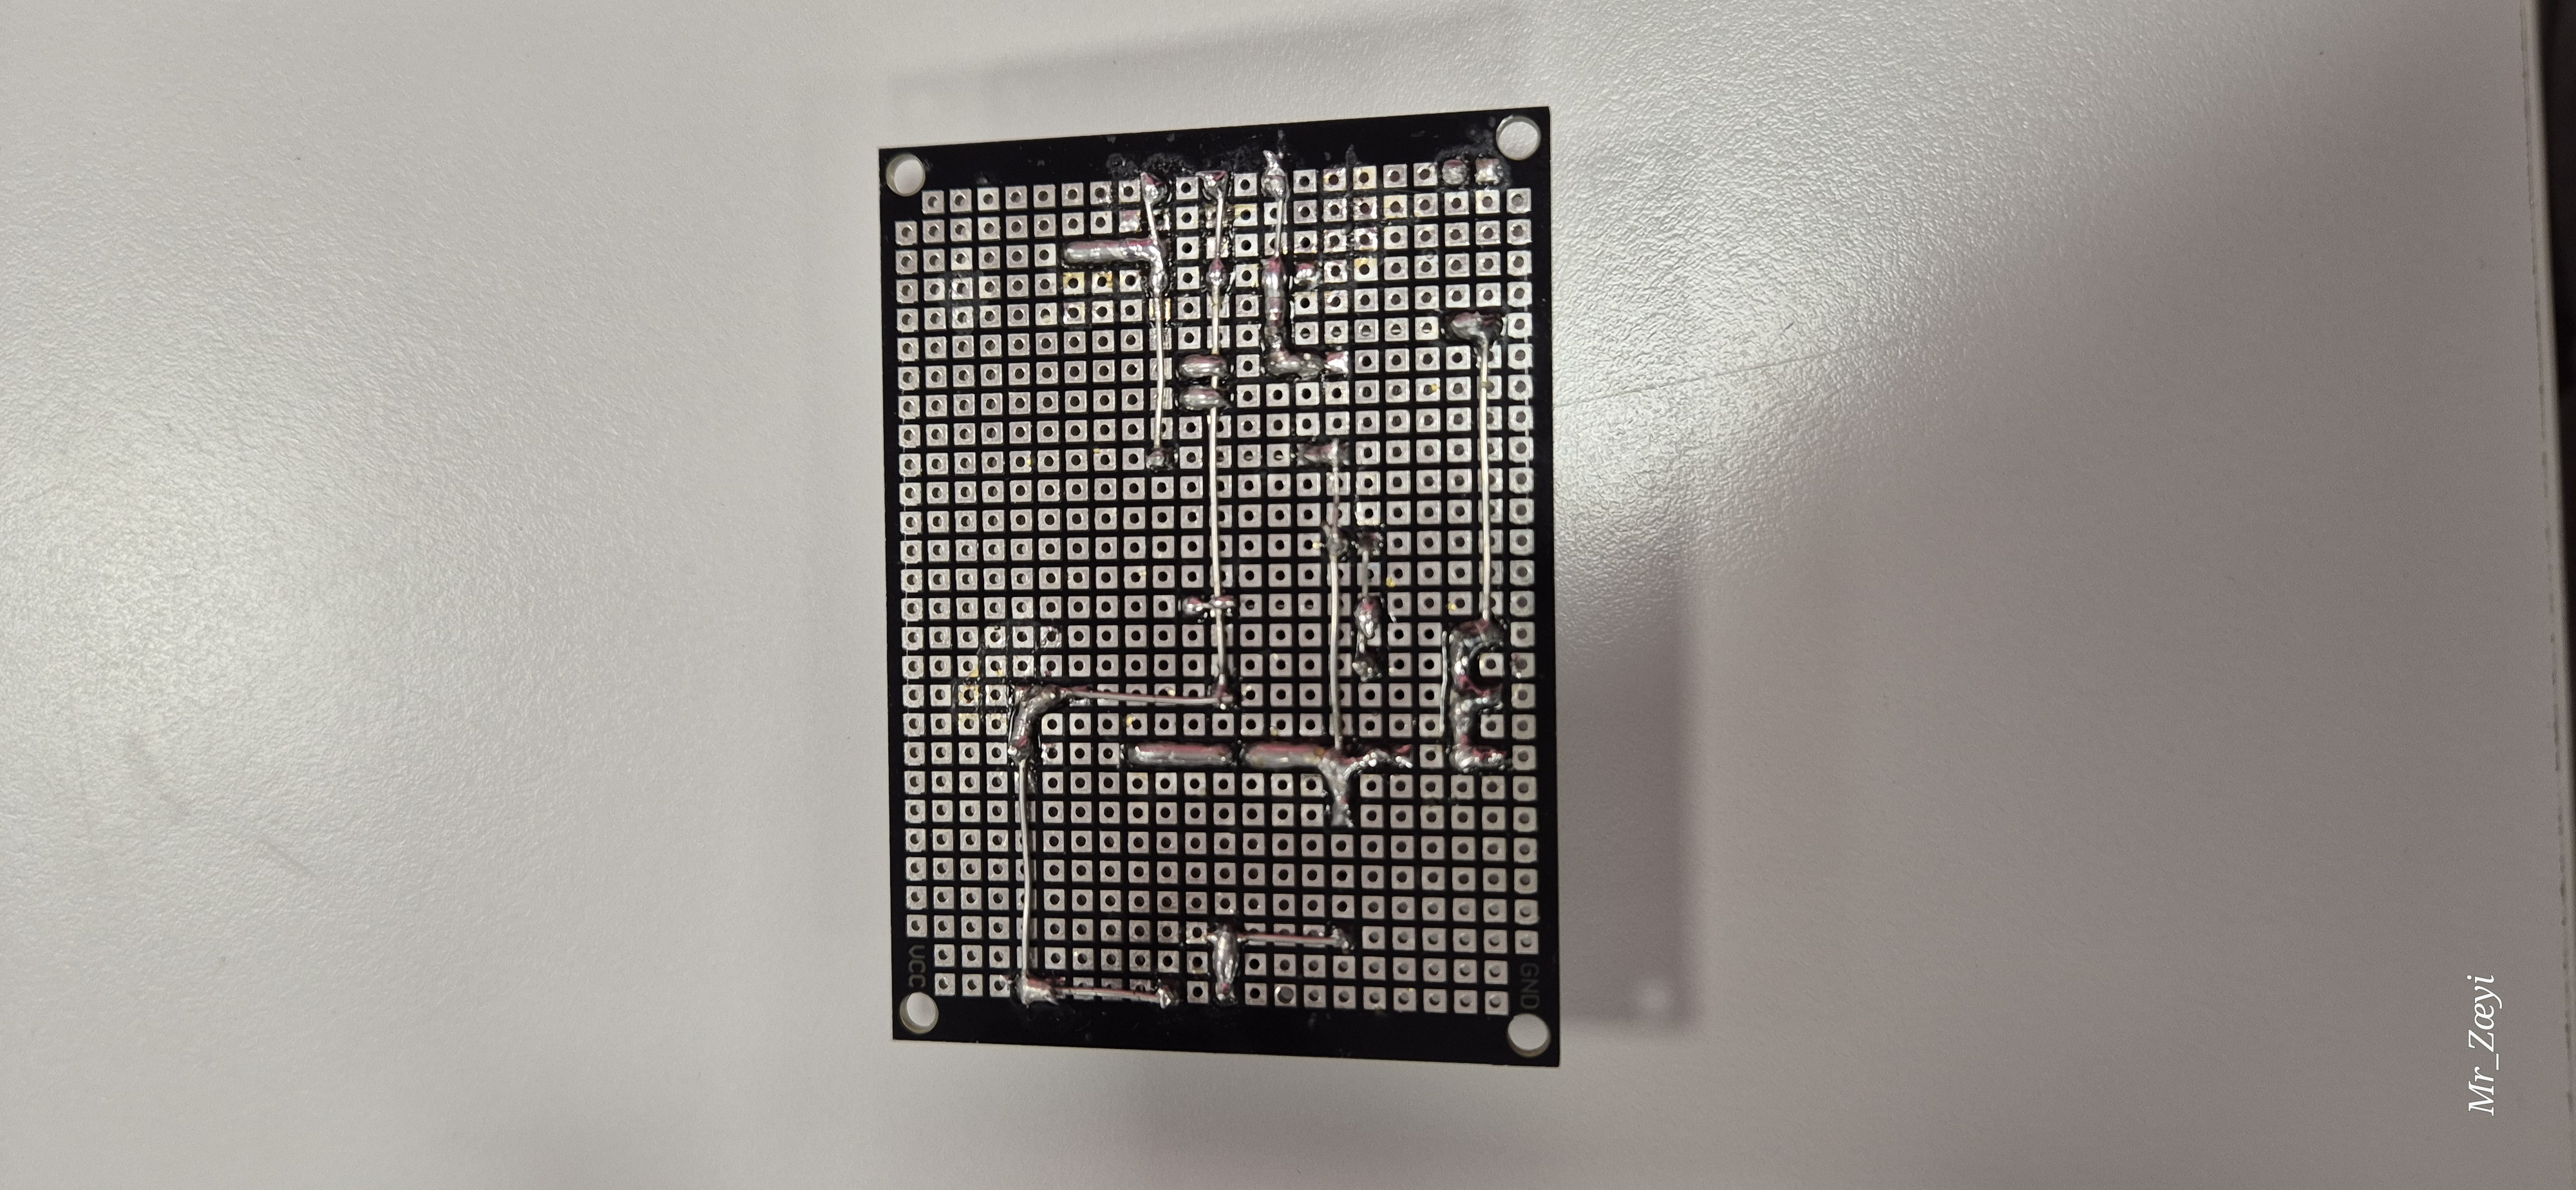
\includegraphics[width=1\textwidth]{20251002_145133.jpg}
    \caption{Carte d’alimentation après soudure et inspection visuelle.}
\end{figure}

\newpage

Une fois la vérification visuelle terminée, la carte a été alimentée en \SI{5.7}{V}. Les tensions de sortie ont été mesurées à l’aide d’un multimètre numérique de précision, d’abord entre les bornes du bornier, puis entre les picots de test afin de vérifier la qualité des soudures et la continuité électrique.

\vspace{0.3cm}
\textbf{Mesures réalisées :}
\begin{itemize}
    \item Tension d’alimentation (V\textsubscript{cc}) : \SI{5=4.99}{V} → écart de \SI{0.2}{\%} par rapport à la valeur attendue.
    \item Référence de tension (V\textsubscript{ref}) : \SI{2.49}{V} → écart de \SI{0.4}{\%}.

\end{itemize}

\begin{figure}[h!]
    \centering
    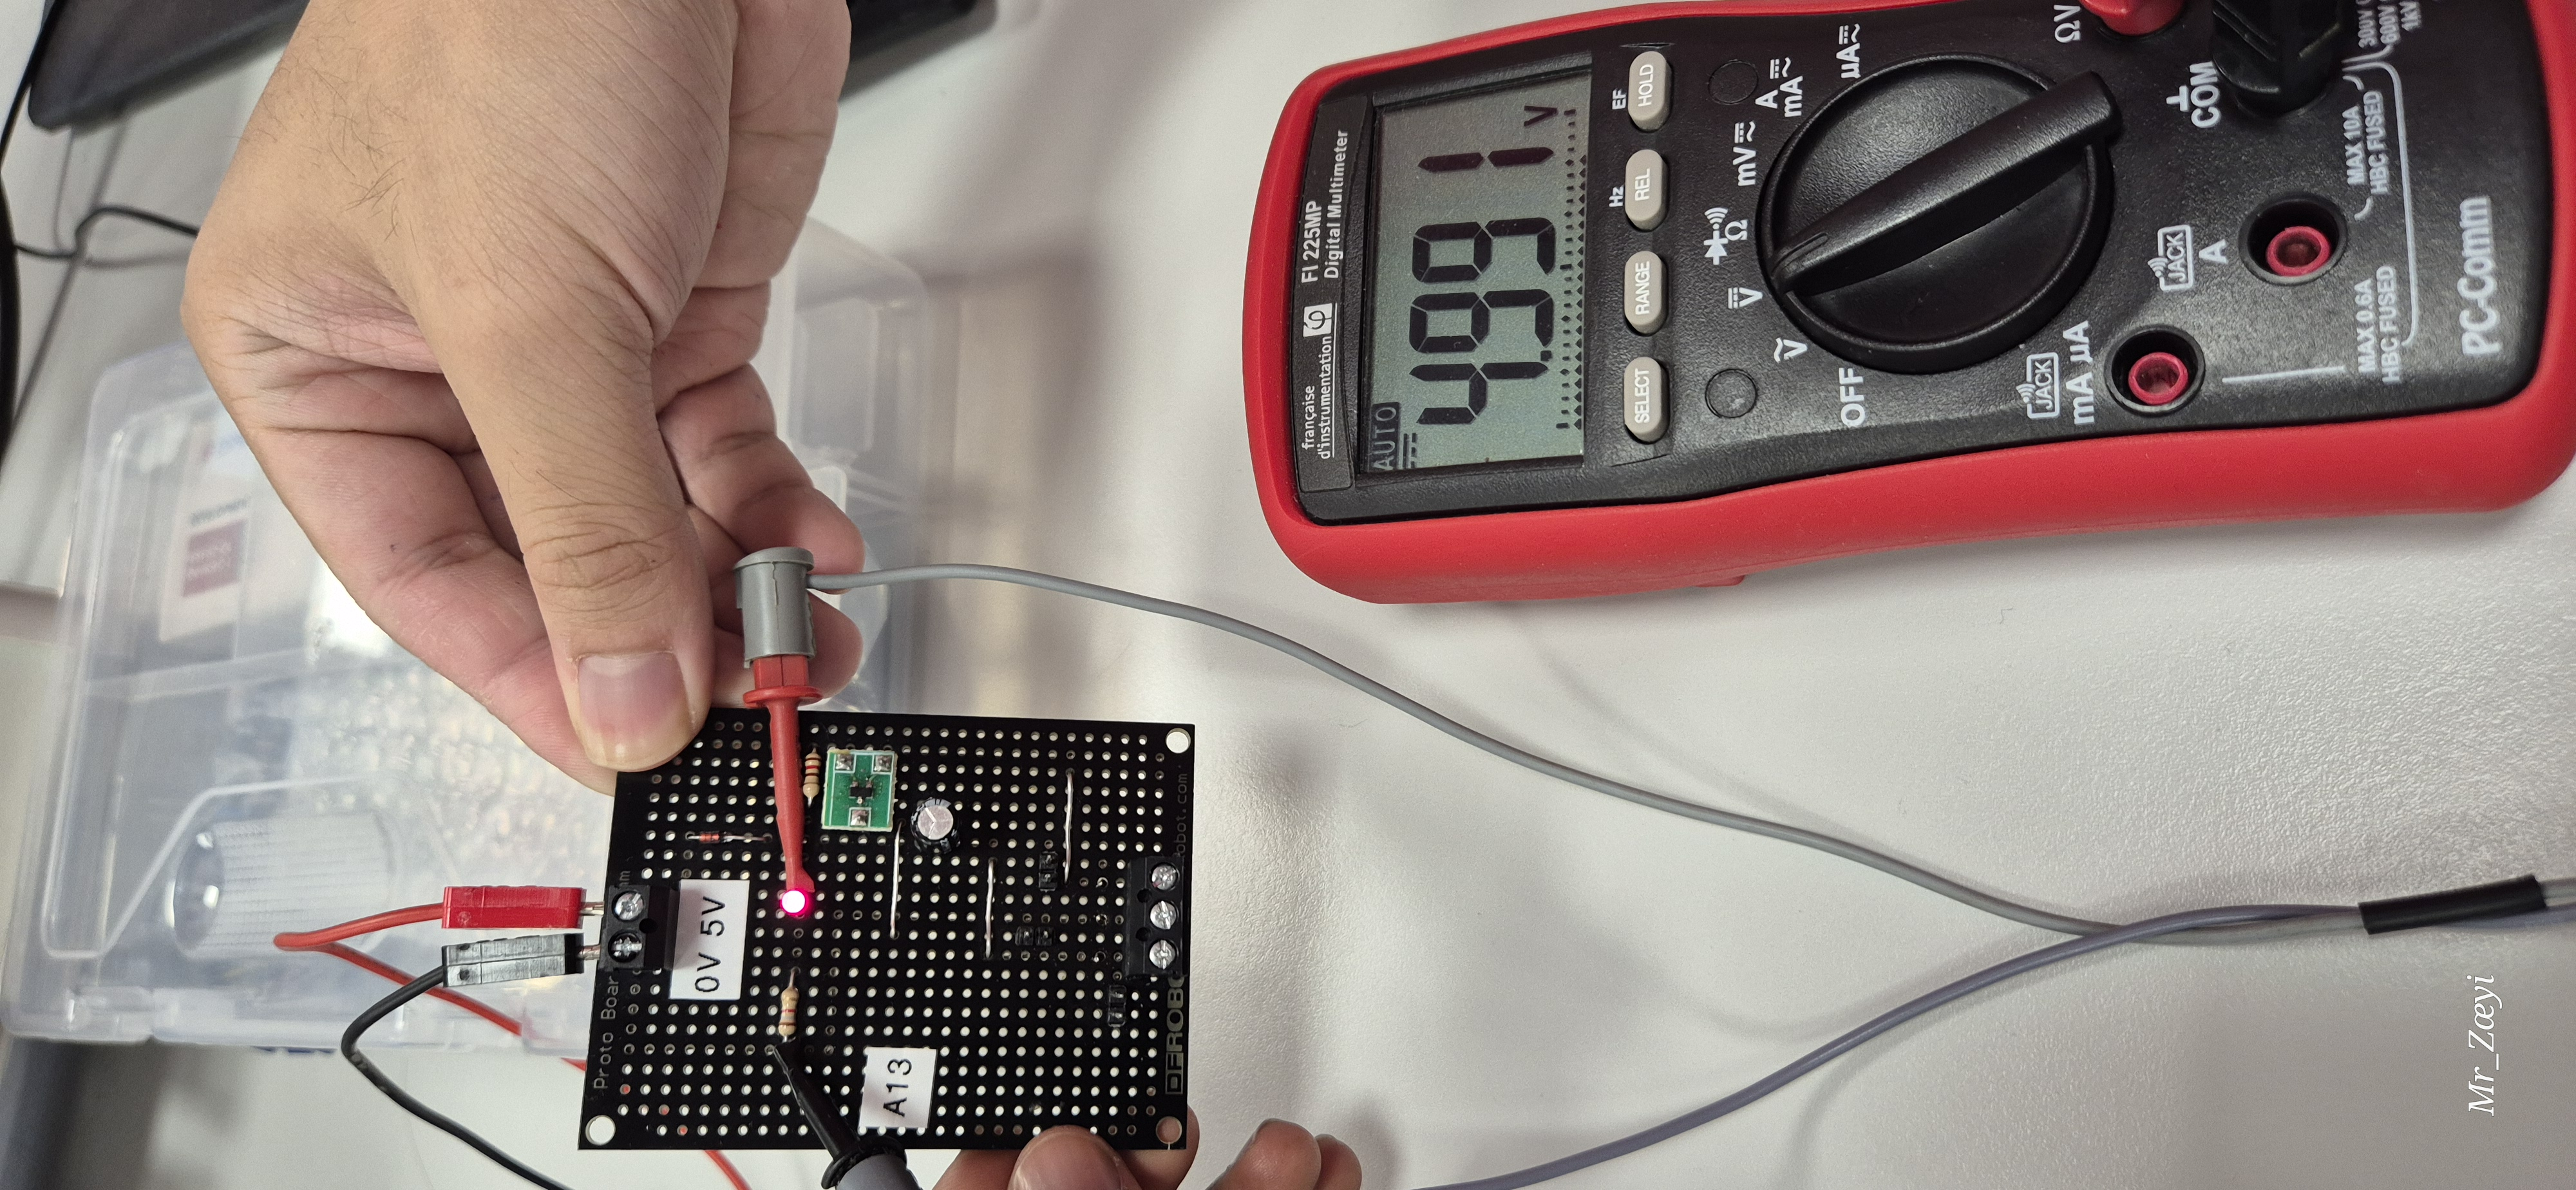
\includegraphics[width=1\textwidth]{20251002_150357 (1).jpg}
    \caption{Mesure de la tension de sortie 5~V avec le multimètre.}
\end{figure}

`\newpage


\subsubsection{Résultats et interprétation}

Les résultats obtenus montrent que les valeurs mesurées respectent les tolérances imposées par le cahier des charges :
\begin{itemize}
    \item La tension de 5~V est stable et conforme à ±0.5~\%.
    \item La tension de référence de 2.5~V est correcte et sans ondulation notable.
    \item L’indicateur LED de mise sous tension fonctionne correctement.
\end{itemize}

Les ondulations observées sont faibles et ne risquent pas de perturber les étages analogiques du système ECG.  
Le filtrage par les condensateurs de découplage s’avère donc efficace.



\subsubsection{Analyse et discussion}

Les écarts mesurés entre les valeurs théoriques et réelles sont très faibles.  
Les éventuelles différences peuvent provenir :
\begin{itemize}
    \item de la tolérance des composants (régulateur, résistances, condensateurs) ;
    \item d’un léger bruit de mesure du multimètre ou de l’oscilloscope ;
    \item de la précision limitée de l’alimentation utilisée (5.7~V ±0.1~V).
\end{itemize}

Aucun problème de polarité ou de soudure n’a été constaté après inspection et mesure.  
La carte est donc jugée fonctionnelle et stable pour alimenter les autres modules du système ECG.

\subsubsection{Conclusion}

La fonction d’alimentation remplit entièrement les exigences du cahier des charges :
\begin{itemize}
    \item Les protections contre les inversions de polarité sont efficaces.
    \item Les tensions de sortie sont conformes et stables.
    \item Le témoin lumineux de mise sous tension est opérationnel.
\end{itemize}

Cette étape validée garantit une base d’alimentation fiable pour les fonctions suivantes du projet, notamment le filtrage et l’amplification du signal ECG.

\newpage

\subsection{Fonction passe-haut à gain variable}

\subsubsection{Introduction à la fonction}

Cette fonction a pour rôle d’amplifier et de filtrer la tension issue de l’étage amplificateur de différence.  
Elle permet d’éliminer la composante continue du signal ECG tout en conservant les variations rapides dues à l’activité cardiaque.  
Le gain de cette fonction doit être ajustable afin d’obtenir, en combinaison avec les autres étages, un gain total compris entre 500 et 1500.

\subsubsection{Rappel du cahier des charges}

La fonction passe-haut à gain variable doit :
\begin{itemize}
    \item réaliser un filtrage passe-haut du premier ordre à une fréquence de coupure de 30~mHz ;
    \item permettre un gain réglable grâce à une résistance variable ;
    \item être implémentée à l’aide d’un amplificateur opérationnel de type MCP6002 ;
    \item fournir une amplification stable et sans distorsion dans la bande utile du signal ECG (0.05~Hz à 150~Hz).
\end{itemize}

\subsubsection{Principe de fonctionnement et dimensionnement}

Le montage retenu est un filtre passe-haut du premier ordre suivi d’un amplificateur non-inverseur à gain variable.  
Le rôle du filtre est d’éliminer la composante continue du signal ECG, tandis que l’amplificateur permet d’ajuster le niveau du signal avant l’étage suivant.

\subsubsection{Calcul de la fréquence de coupure}

Le condensateur \( C \) du filtre a une valeur imposée de \( 3.3~\mu F \).  
La résistance \( R \) associée a été calculée afin d’obtenir une fréquence de coupure de :

\[
f_c = \frac{1}{2\pi R C}
\]

En isolant \( R \) :

\[
R = \frac{1}{2\pi f_c C} = \frac{1}{2\pi \times 0.03 \times 3.3 \times 10^{-6}} \approx 1.6~M\Omega
\]

Ainsi, la fréquence de coupure est bien d’environ \( 30~\text{mHz} \), conforme au cahier des charges.
On choisit la valeur normalisée la plus proche, soit R = 1.5M $\Omega$ .

Avec cette résistance, notre fréquence de coupure est égale à :
\begin{equation}
    f_c = \frac{1}{2 \pi RC} = \frac{1}{2 \pi \times 1.5M \times 3.3 \times 10^-6} = 32.1 mHz
\end{equation}

Sur la simulation, notre fréquence de coupure est à 33.1 mHz.

\subsubsection{Principe d’amplification}

L’amplification est assurée par un amplificateur opérationnel \textbf{MCP6002}, monté en suiveur pour garantir une impédance d’entrée élevée et isoler le filtre du reste du montage.  
Le gain variable est ensuite obtenu à l’aide d’un montage non-inverseur, selon la relation :

\[
G = 1 + \frac{R_f}{R_{in}}
\]

La résistance \(R_f\) est composée d’une résistance fixe de \(47~k\Omega\) (imposée) en série avec une résistance variable \(R_{var}\).  
La résistance \(R_{in}\) est à déterminer de façon à obtenir un gain minimal de 10 lorsque \(R_{var} = 0~\Omega\).

\subsubsection{Détermination de \(R_{in}\)}

\[
G_{min} = 1 + \frac{R_f}{R_{in}} = 10
\Rightarrow R_{in} = \frac{R_f}{G_{min}-1} = \frac{47k}{9} = 5.22~k\Omega
\]

On choisit la valeur normalisée la plus proche, soit \(R_{in} = 5.1~k\Omega\).

Avec cette valeur, nous devrions avoir un gain égal à:
\begin{equation}
    G_{min}=1+\frac{R_{f}}{R_{in}}= 1+ \frac{47k}{5.1k} =10.21 
\end{equation}
Le choix de cette résistance est pertinant puisqu'elle nous permet de rester dans la plage de gain demandé.
\subsubsection{Détermination de la résistance variable maximale}

On souhaite un gain maximal de \(G_{max} = 30\).  
En isolant \(R_{var}\) :

\[
R_{var} = (G_{max}-1)\,R_{in} - 47k
\]

\[
R_{var,\max} = (30-1)\times5.1k - 47k = 147.9k - 47k \approx 100.9~k\Omega
\]
Si on choisit un potentiomètre variant de 0 à 100k $\Omega$ on a :
\begin{equation}
    G_{max}=1+\frac{R_{f}+R_{var,max}}{R_{in}} = 1 + \frac{47k+100k}{5.1k}=29.82
\end{equation}
Un potentiomètre de \(100~k\Omega\) est donc parfaitement adapté, permettant d’obtenir un gain variant de 10.21 à environ 29.82.  
Cette plage respecte les contraintes du cahier des charges et s’intègre dans le gain global souhaité du système ECG (500 à 1500 pour la chaîne complète).

\begin{figure}[h!]
    \centering
    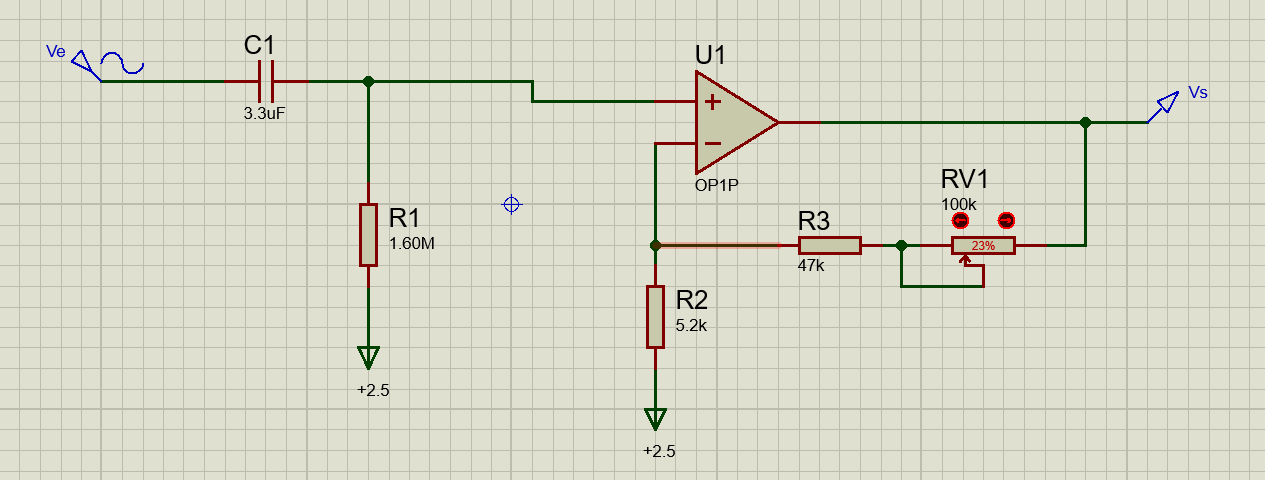
\includegraphics[width=0.7\textwidth]{schematic_simu.png}
    \caption{Schéma électrique du filtre passe-haut à gain variable réalisé sous Proteus.}
\end{figure}

\subsubsection*{Simulation}

Avant la réalisation pratique, une simulation complète du montage a été effectuée sous Proteus afin de vérifier le comportement du filtre passe-haut à gain variable.  
Les objectifs principaux de cette simulation étaient :
\begin{itemize}
    \item valider la fréquence de coupure à \textbf{30~mHz} ;
    \item observer la variation de gain entre la position minimale et maximale du potentiomètre ;
\end{itemize}

\subsubsection{Fréquence de coupure}

La première simulation consiste à observer la réponse fréquentielle du filtre.  
La courbe de Bode montre une atténuation de \(-3~\text{dB}\) autour de \textbf{30~mHz}, ce qui correspond bien à la fréquence de coupure calculée théoriquement.

\begin{figure}[h!]
    \centering
    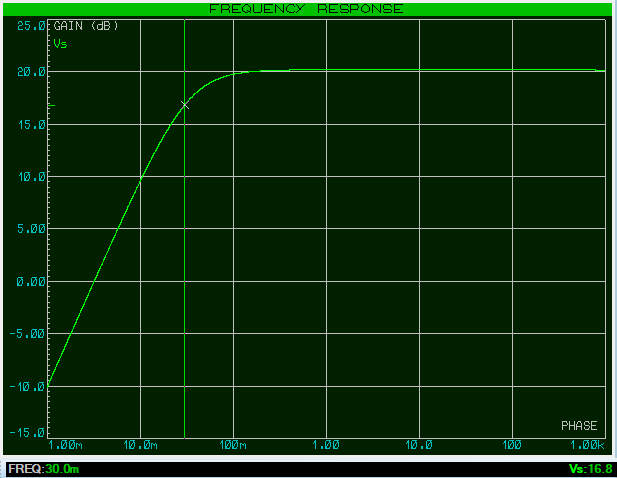
\includegraphics[width=0.75\textwidth]{frec_coup.png}
    \caption{Simulation de la fréquence de coupure du filtre passe-haut (\(f_c \approx 30~\text{mHz}\)).}
\end{figure}

\newpage

\subsubsection{Gain minimal}

Une seconde simulation a été réalisée avec la résistance variable réglée à \(R_{var} = 0~\Omega\), correspondant au \textbf{gain minimal} (\(G \approx 10.23\)) ce qui est cohérent à coté du gain théorique (\(G \approx 10.21\))
Le signal de sortie reste faible mais propre, sans distorsion notable.

\begin{figure}[h!]
    \centering
    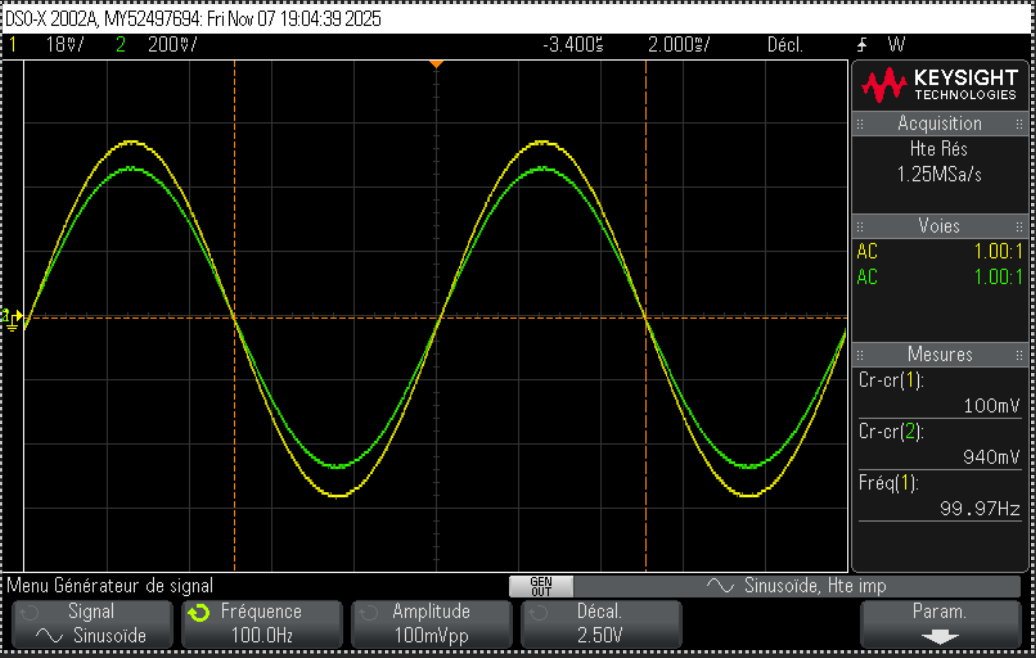
\includegraphics[width=0.75\textwidth]{gain_min.png}
    \caption{Simulation du signal de sortie pour le gain minimal (\(G \approx 10.23\)).}
\end{figure}

\newpage

\subsubsection{Gain maximal}

Enfin, la simulation du montage avec la résistance variable réglée à sa valeur maximale (\(R_{var} = 100~k\Omega\)) permet d’observer le \textbf{gain maximal} (\(G \approx 29.85\)). Toujours cohérent comparé au gain théorique ((\(G \approx 29.82\)) 
Le signal de sortie est amplifié correctement et reste dans la plage linéaire de fonctionnement de l’AOP.

\begin{figure}[h!]
    \centering
    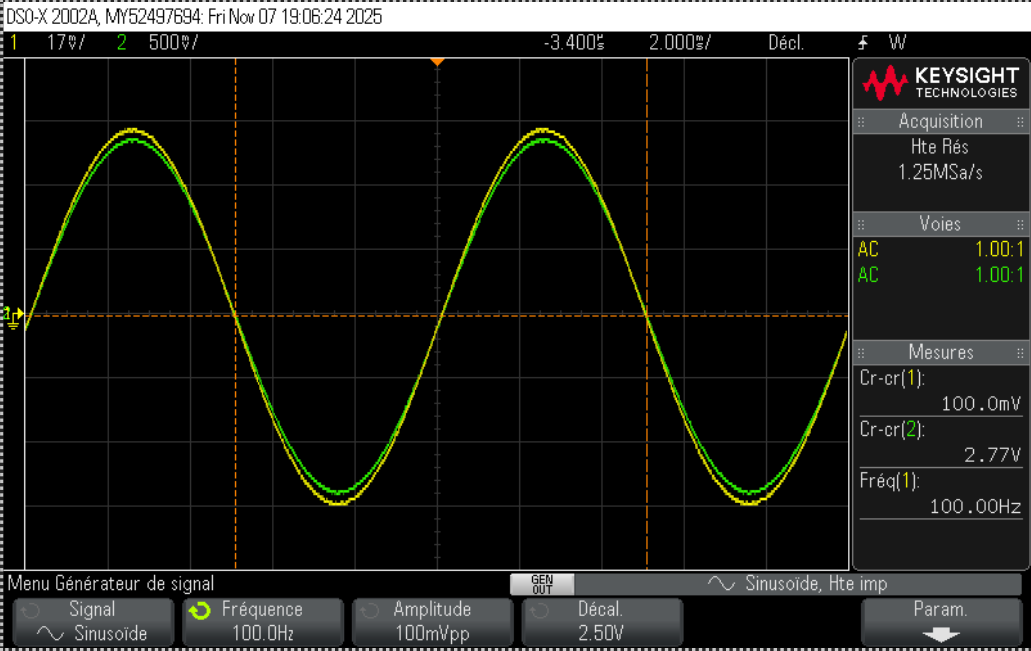
\includegraphics[width=0.75\textwidth]{gain_max.png}
    \caption{Simulation du signal de sortie pour le gain maximal (\(G \approx 29.58\)).}
\end{figure}
\newpage

\subsubsection{Analyse}

Les résultats obtenus en simulation sont cohérents avec les calculs théoriques :
\begin{itemize}
    \item la fréquence de coupure correspond bien à 30~mHz ;
    \item la variation de gain observée est conforme à la plage prévue ;
    \item aucune instabilité ni saturation de l’amplificateur n’a été constatée.
\end{itemize}

Ces simulations confirment la validité du dimensionnement du filtre passe-haut à gain variable avant la phase de réalisation pratique.

\subsubsection{Composants nécessaires}

La liste complète des composants pour réaliser la fonction passe-haut à gain variable est la suivante :

\begin{table}[h!]
\centering
\caption{Liste des composants de la fonction passe-haut à gain variable}
\begin{tabular}{|c|c|c|}
\hline
\textbf{Référence} & \textbf{Désignation} & \textbf{Valeur / Type} \\
\hline
VE\_PHGB & Connecteur d’entrée & 2 broches \\
\hline
C\_PH\_1 & Condensateur & 3.3~µF \\
\hline
R\_PH\_1 & Résistance & 1.5~MΩ \\
\hline
GAIN\_VAR:B & Amplificateur opérationnel & MCP6002 \\
\hline
R\_VAR\_1 & Résistance d’entrée & 5.1~kΩ \\
\hline
R\_VAR & Résistance de contre-réaction & 47~kΩ \\
\hline
RV1 & Potentiomètre & 100~kΩ \\
\hline
C\_DEC\_PASSE\_HAUT & Condensateur de découplage & 100~nF \\
\hline
VS\_PHGV & Connecteur de sortie & 2 broches \\
\hline
\end{tabular}
\end{table}

\newpage

\subsubsection{Réalisation et état d’avancement}

La conception et la simulation du montage sont terminées.  
La carte a été implantée virtuellement sur Proteus (version PCB) et les composants nécessaires ont été sélectionnés : condensateur \(3.3~\mu F\), résistances fixes et potentiomètre de \(100~k\Omega\).  
La phase de soudure est en cours de réalisation.  

Les prochaines étapes seront :
\begin{itemize}
    \item terminer la soudure du montage sur protoboard ;
    \item effectuer un contrôle visuel et vérifier la continuité des pistes ;
    \item mesurer expérimentalement la fréquence de coupure et le gain pour différentes valeurs de \(R_{var}\) ;
    \item comparer les résultats expérimentaux aux valeurs simulées.
\end{itemize}

\begin{figure}[h!]
    \centering
    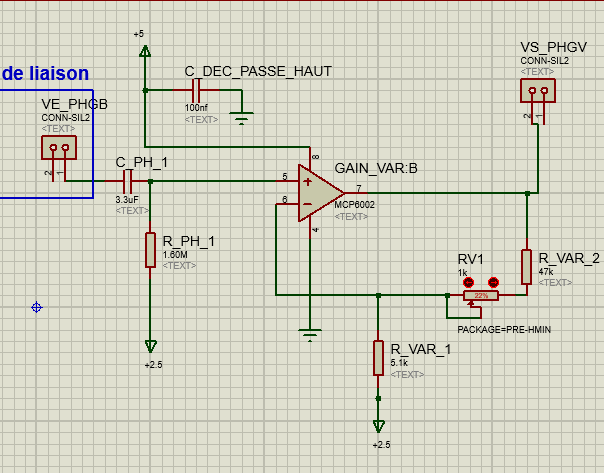
\includegraphics[width=1\textwidth]{schematic_PH.png}
    \caption{Implantation de la fonction passe-haut à gain variable avant soudure.}
\end{figure}

\begin{figure}[h!]
    \centering
    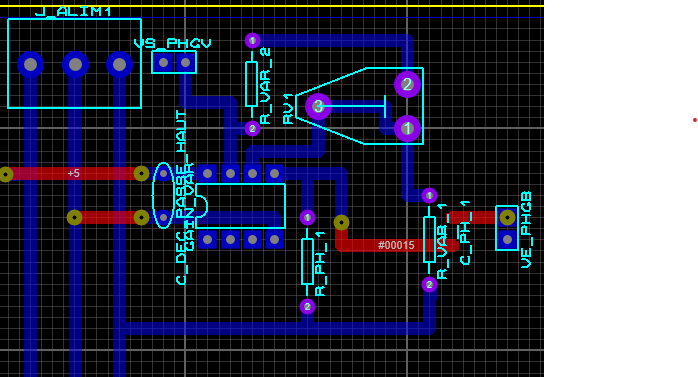
\includegraphics[width=1\textwidth]{PCB_final.png}
    \caption{Implantation PCB de la fonction passe-haut à gain variable sur Proteus .}
\end{figure}

\newpage

\subsubsection{Conclusion}

La conception théorique et la simulation de la fonction passe-haut à gain variable sont conformes au cahier des charges.  
Les calculs de dimensionnement ont permis de fixer les valeurs suivantes :
\begin{itemize}
    \item \(C = 3.3~\mu F\) ;
    \item \(R = 1.5~M\Omega\) pour une coupure à 30~mHz ;
    \item \(R_{in} = 5.1~k\Omega\) ;
    \item \(R_f = 47~k\Omega + R_{var}\), avec \(R_{var}\) variant de 0 à \(100~k\Omega\).
\end{itemize}

Les simulations montrent un gain variable de 10 à 30 et un comportement fréquentiel stable.  
La soudure et les tests expérimentaux viendront confirmer la validité du montage et sa conformité au cahier des charges global du projet ECG.

\subsubsection{Tests expérimentaux et analyse des résultats}

Après la phase de conception et de simulation, la fonction passe-haut à gain variable a été réalisée sur platine (protoboard) puis testée expérimentalement.
\begin{figure}[h!]
    \centering
    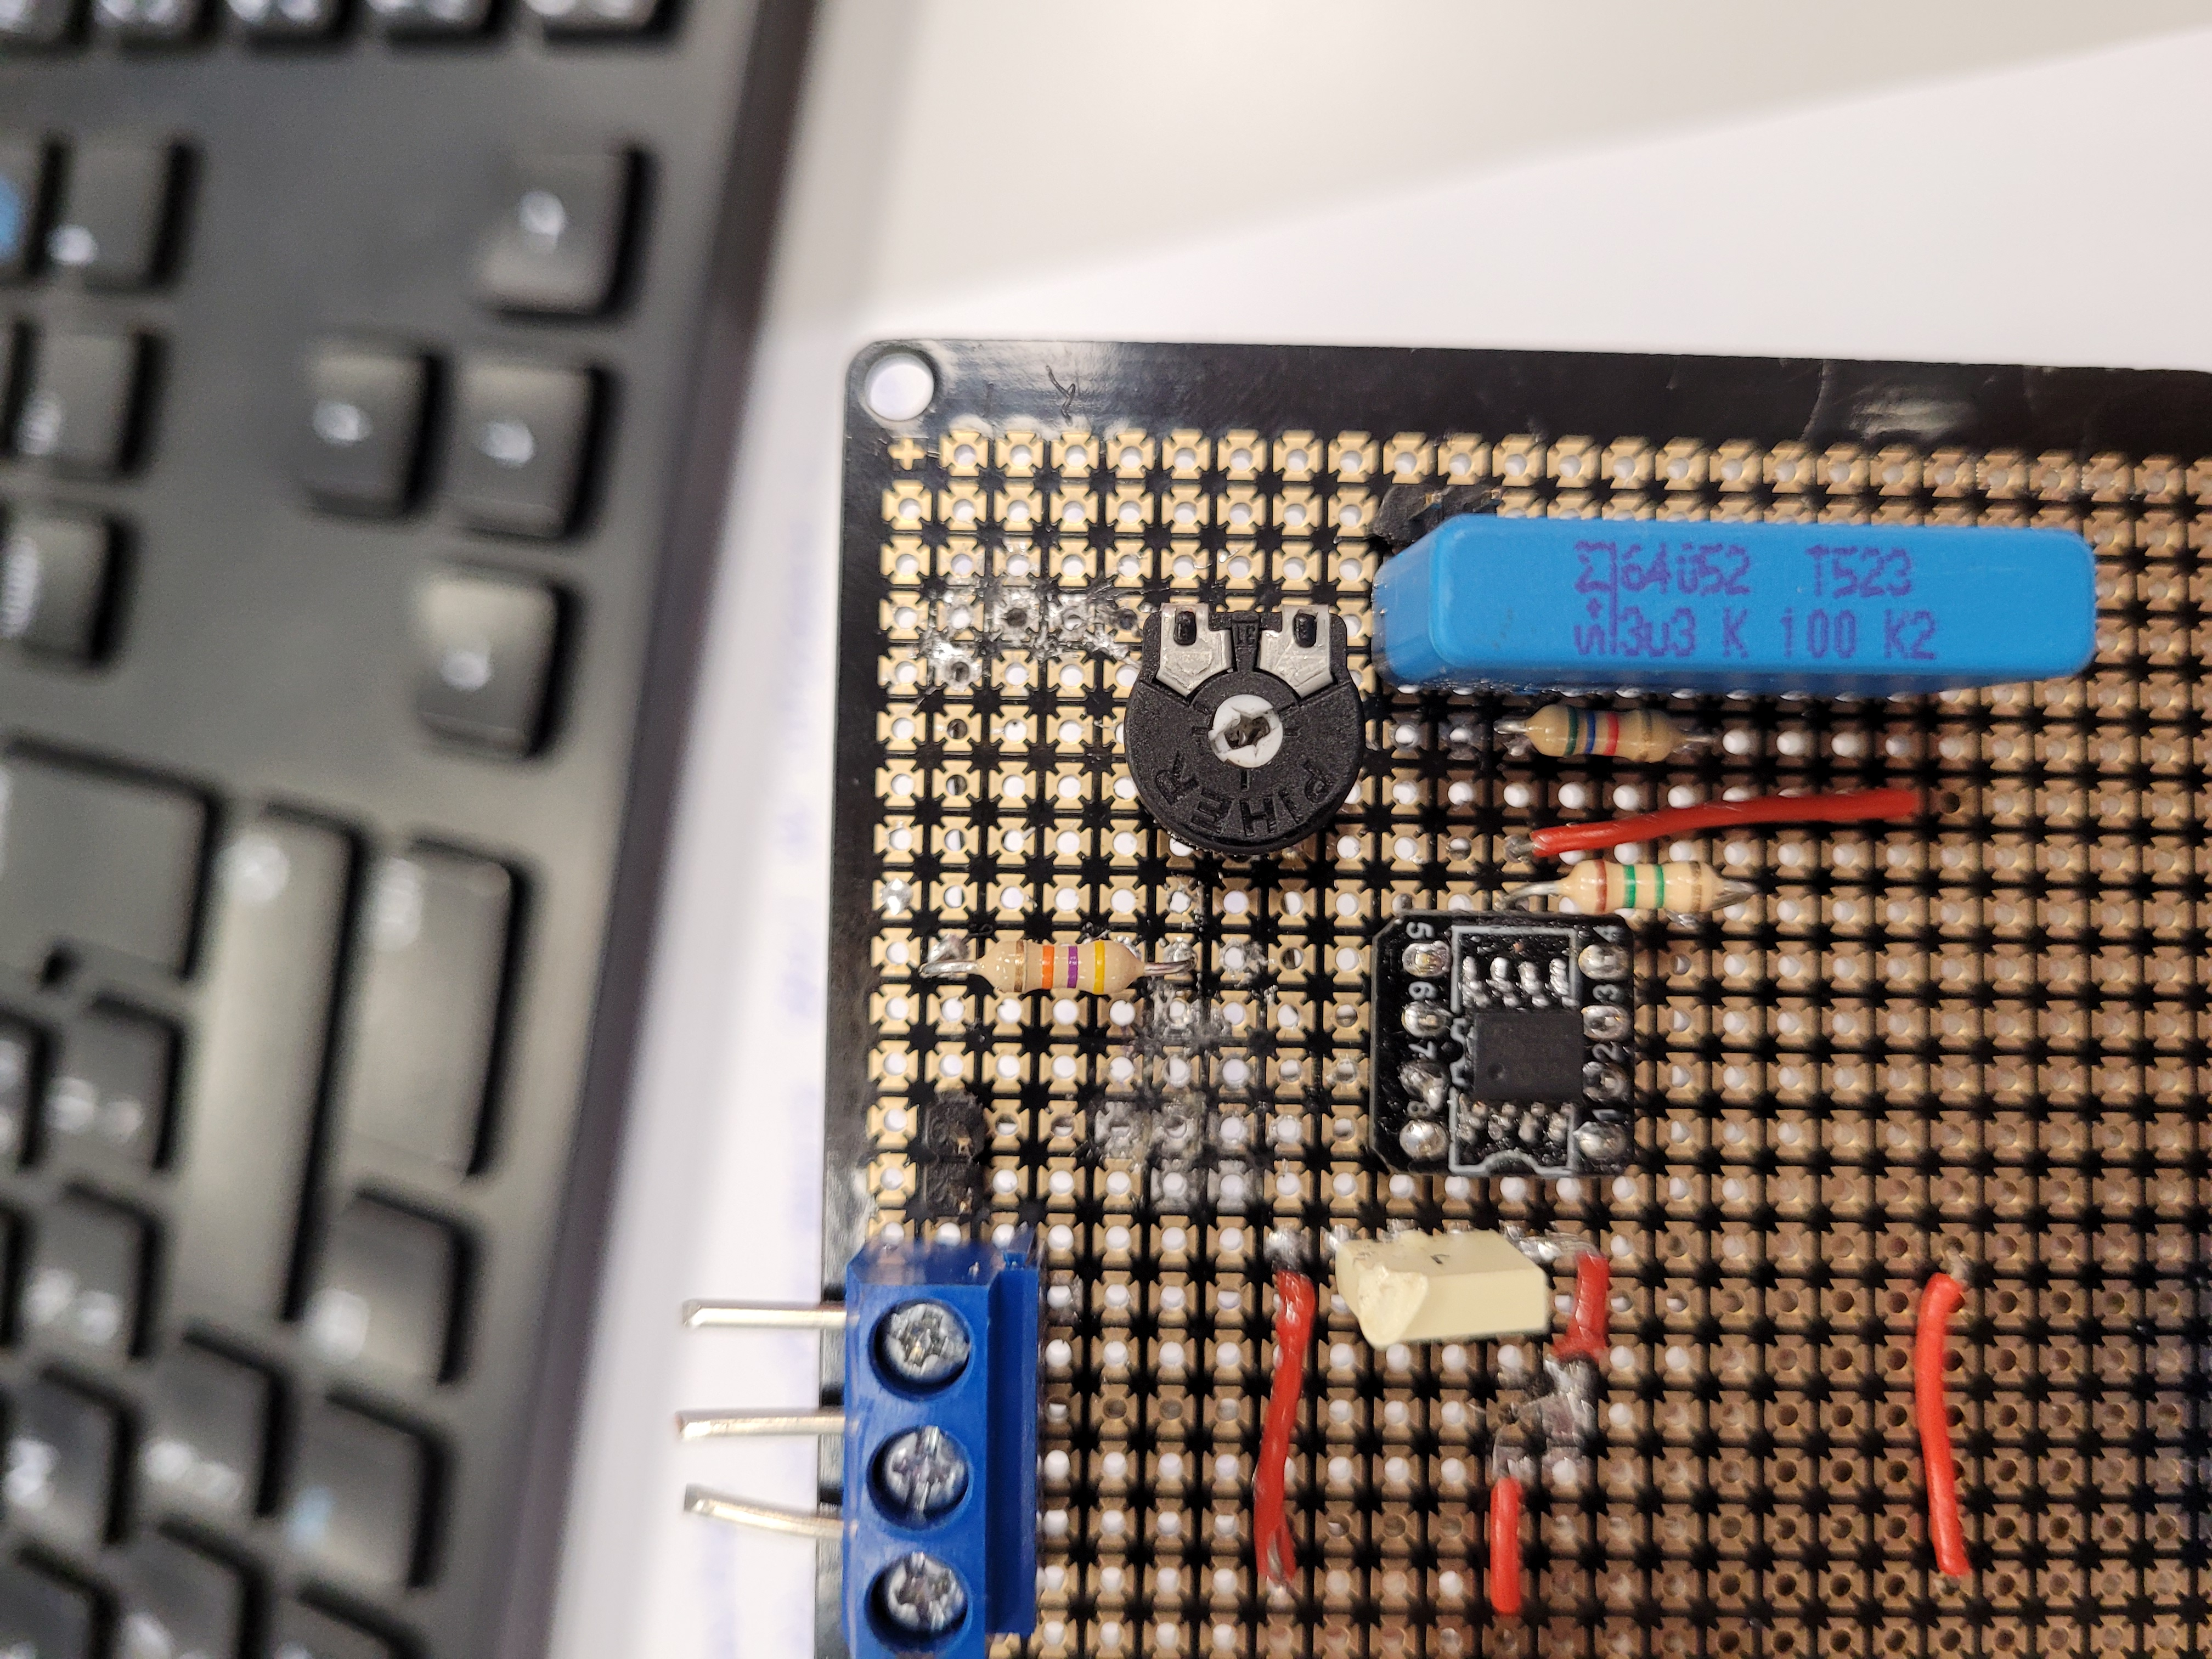
\includegraphics[width=0.75\textwidth]{realisation_sur_platine1.jpg}
    \caption{Réalisation de la fonction passe-haut à gain variable (dessus)}
\end{figure}

\begin{figure}[h!]
    \centering
    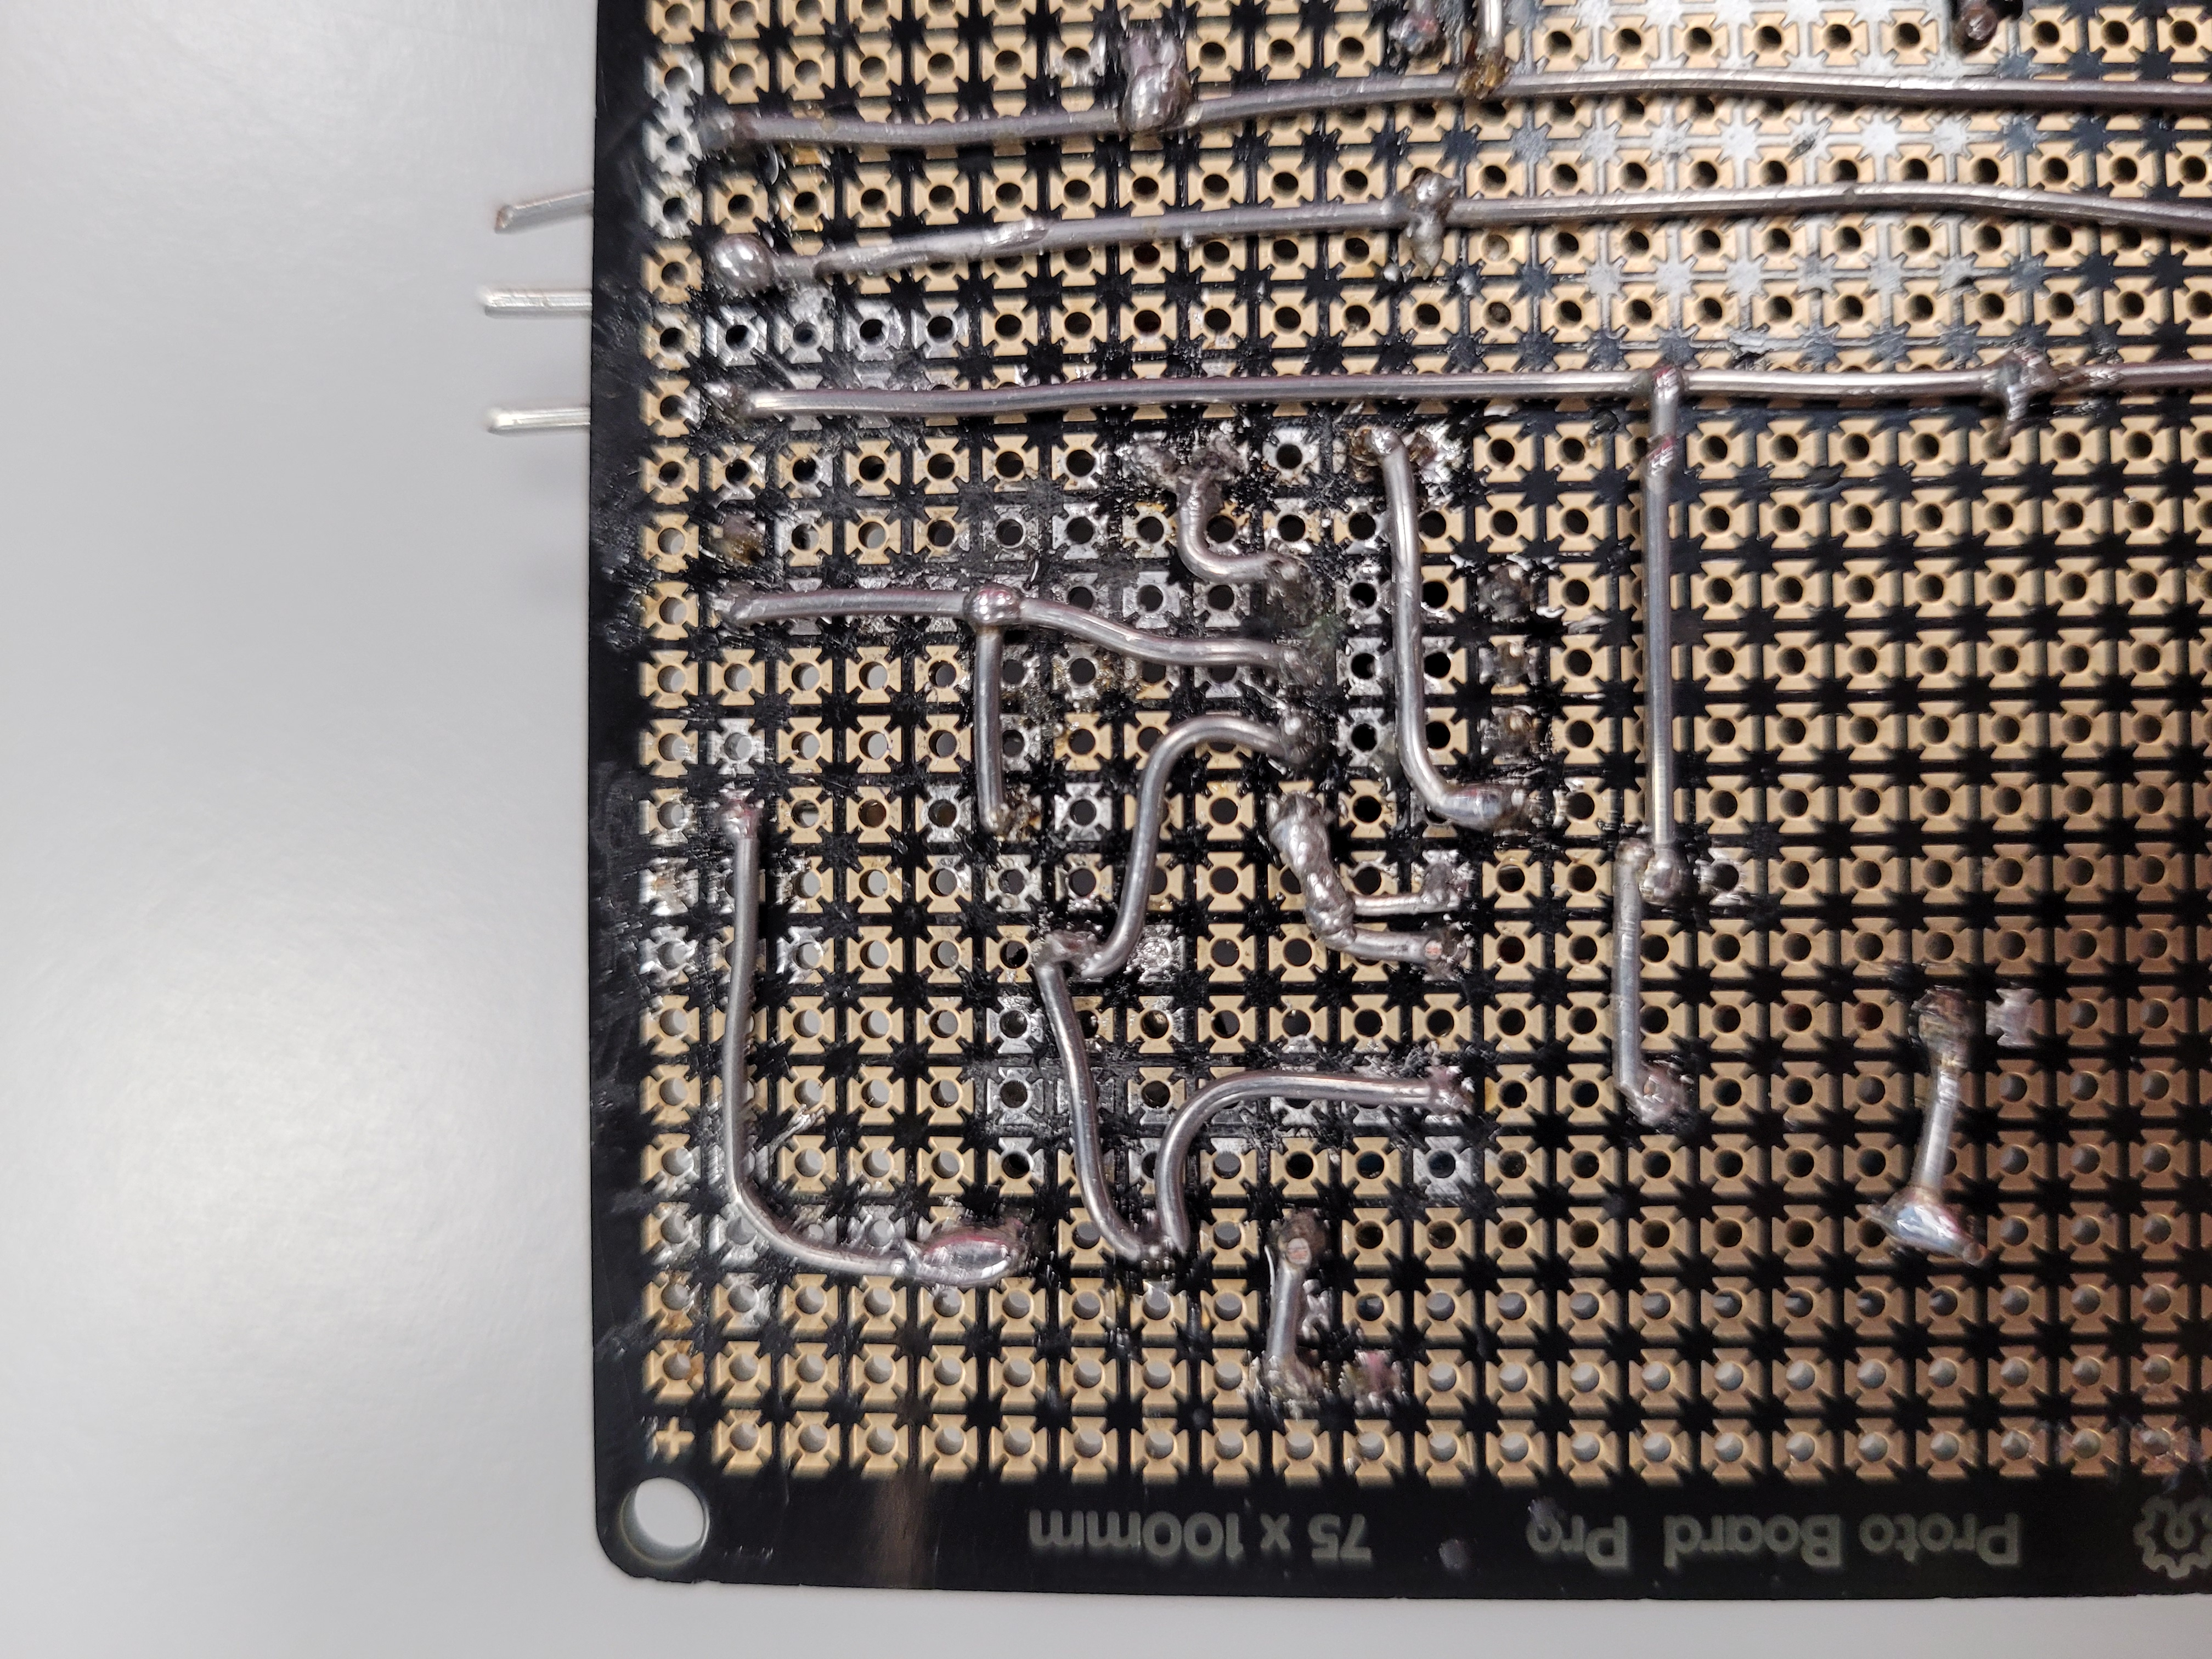
\includegraphics[width=0.75\textwidth]{realisation_sur_platine2.jpg}
    \caption{Réalisation de la fonction passe-haut à gain variable (dessous) }
\end{figure}

\newpage

L’objectif de cette étape était de vérifier que le montage respecte les caractéristiques prévues : fréquence de coupure, plage de gain, et stabilité du signal.

\subsubsection{Mise en place du banc de test}

Le montage a été alimenté en \(+5~\text{V}\) à partir de la carte d’alimentation du projet.  
Les signaux d’entrée ont été fournis par un générateur de fonctions basse fréquence (GBF) configuré pour délivrer une tension sinusoïdale d’amplitude \textbf{100~mV crête-à-crête} avec un \textbf{offset de 2.5~V}.  
Cet offset est indispensable car le montage est alimenté en \(5~\text{V}\) simple et utilise une tension de référence de \(2.5~\text{V}\) : il permet donc de centrer le signal dans la zone linéaire de fonctionnement de l’amplificateur opérationnel MCP6002 et d’éviter toute saturation.  

L’amplitude d’entrée de \textbf{100~mV\(_{pp}\)} a été choisie car elle correspond à l’ordre de grandeur du signal ECG réel mesuré par les électrodes (quelques millivolts après l’étage différentiel) et reste suffisamment faible pour garantir un fonctionnement en régime linéaire de l’amplificateur.  
Cette faible amplitude permet également de tester la sensibilité et la stabilité du montage sans risquer de saturer l’étage de sortie ou de fausser la mesure du gain.
 
Cet offset est indispensable car le montage est alimenté en 5~V simple et utilise une tension de référence de 2.5~V : il permet donc de centrer le signal dans la zone linéaire de fonctionnement de l’amplificateur opérationnel MCP6002 et d’éviter toute saturation.

Les mesures ont été effectuées à l’aide d’un oscilloscope numérique double voie, en comparant la tension d’entrée et la tension de sortie pour différentes fréquences et positions du potentiomètre.  
Les composants montés sont conformes au dimensionnement théorique :

\begin{itemize}
    \item \(C = 3.3~\mu F\),
    \item \(R = 1.5~M\Omega\),
    \item \(R_{in} = 5.1~k\Omega\),
    \item \(R_f = 47~k\Omega + R_{var}\) (potentiomètre de \(100~k\Omega\)).
\end{itemize}




\subsubsection{Mesure de la fréquence de coupure}

Conformément aux consignes de la fiche de fonction, la fréquence de coupure a été déterminée expérimentalement à partir de la mesure de la tension de sortie \(V_S\) pour les deux valeurs extrêmes du gain (\(G_{min}\) et \(G_{max}\)).  

Le principe de mesure consiste à injecter un signal sinusoïdal d’amplitude constante et à faire varier la fréquence jusqu’à obtenir une atténuation de \(0.707 \times V_{S,0}\) (soit \(-3~\text{dB}\)).  
Cette fréquence correspond à la fréquence de coupure \(f_c\) du filtre passe-haut.

\textbf{Cas 1 – Gain minimal (\(G \approx 10\)) :}

\begin{figure}[H]
    \centering
    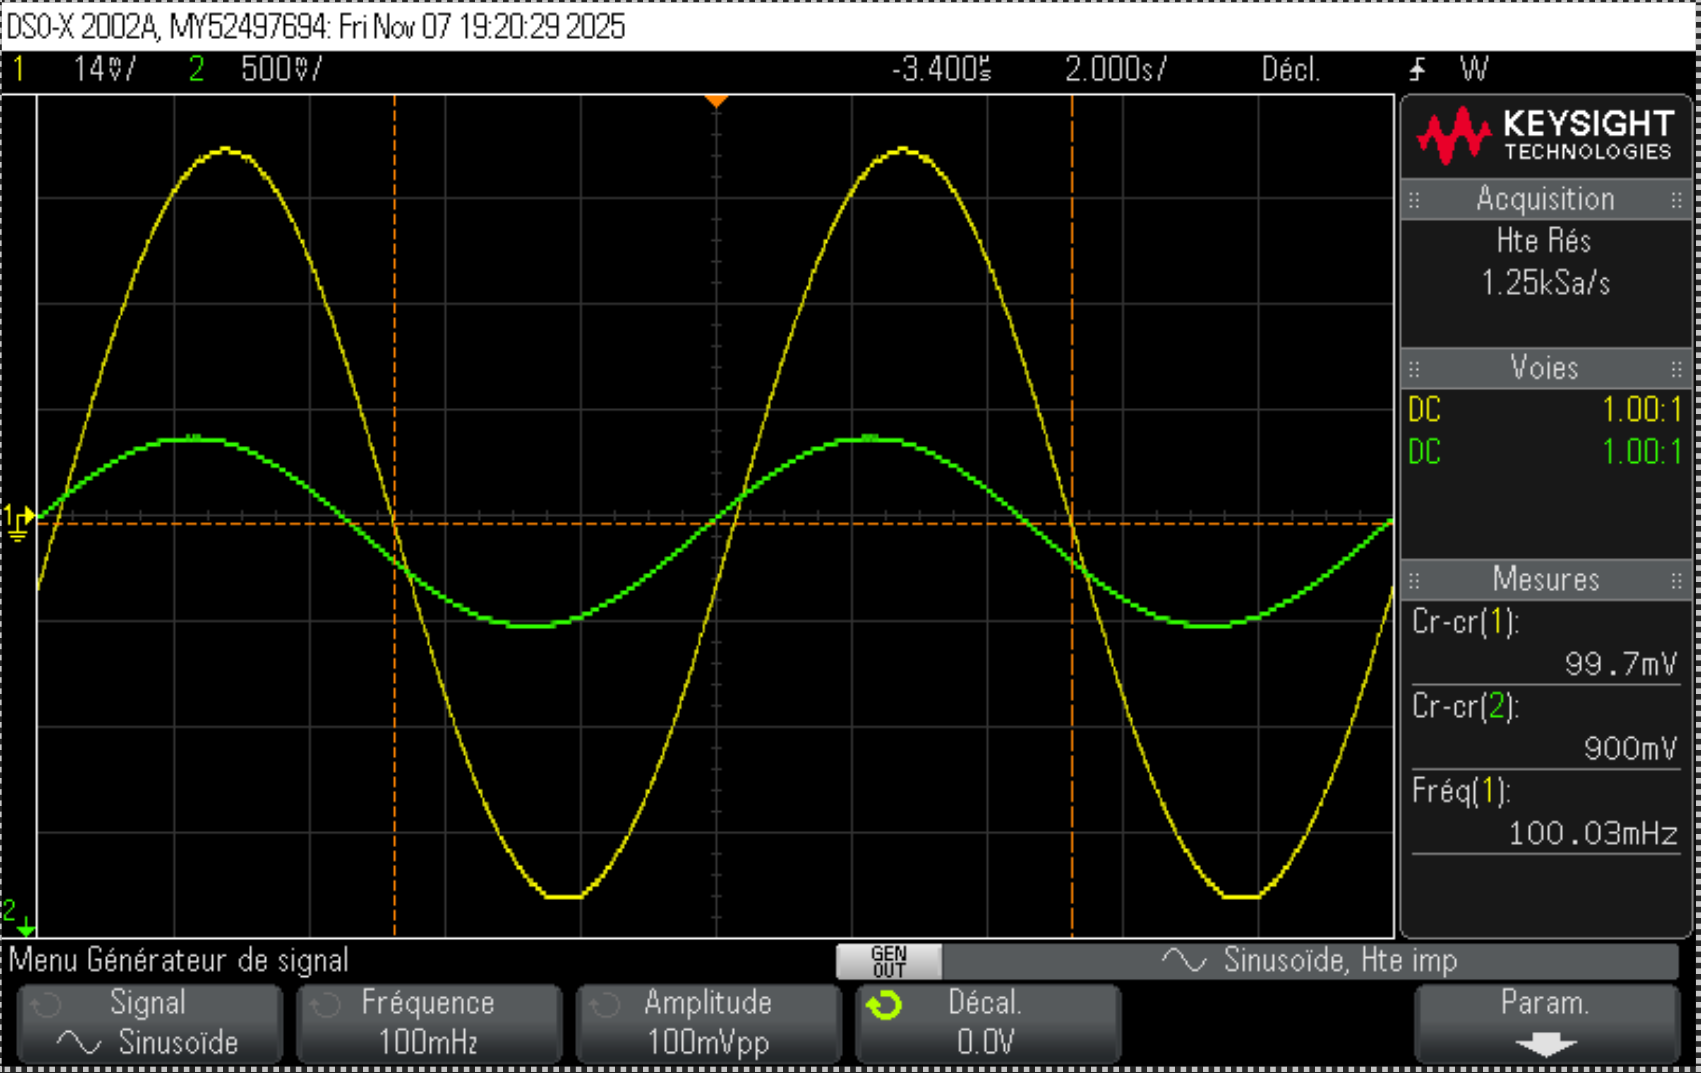
\includegraphics[width=0.75\textwidth]{gain_min_freq_100mhz.png}
    \caption{Mesure de la fréquence de coupure à faible gain (\(G_{min} \approx 10\)).}
\end{figure}

La fréquence de coupure observée est conforme à la valeur théorique d’environ 30~mHz.  
Le diagramme de Bode correspondant à ce réglage de gain confirme une atténuation de \(-3~\text{dB}\) à la même fréquence.

\begin{figure}[H]
    \centering
    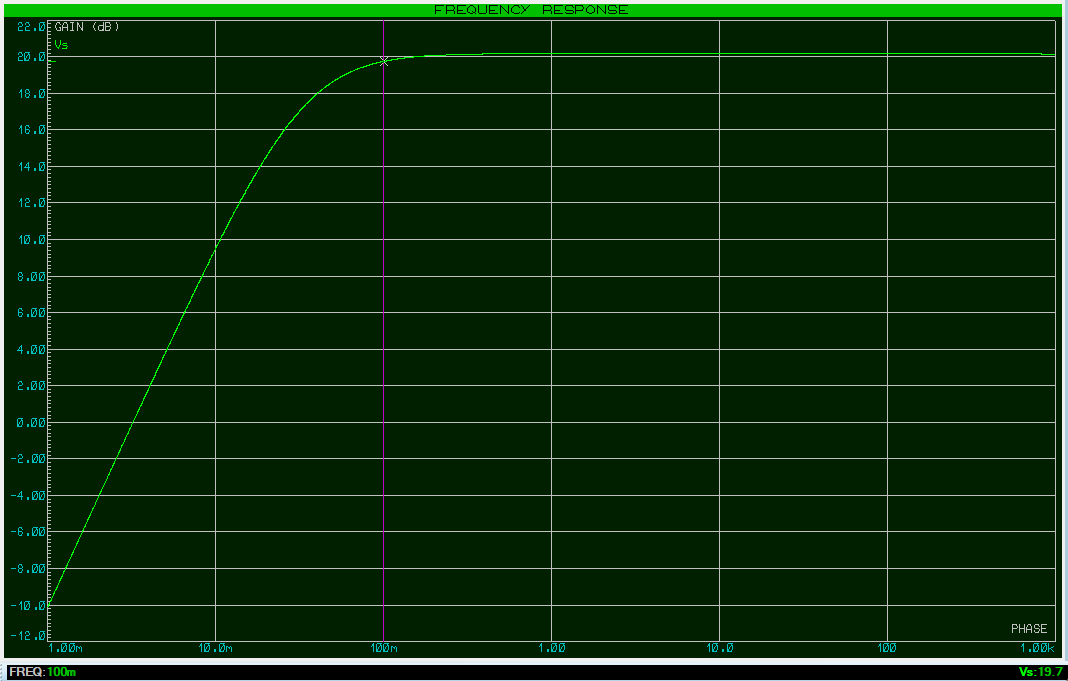
\includegraphics[width=1\textwidth]{Gain_a_100mHZ_potento_min.png}
    \caption{Diagramme de Bode simulé sous Proteus pour le gain minimal (\(G_{min} \approx 10\)).}
\end{figure}

\paragraph{Analyse des tolérances — Gain minimal}

Pour \(R_{var} = 0~\Omega\), le gain dépend uniquement du rapport \(\frac{R_f}{R_{in}}\).  
Avec \(R_f = 47~k\Omega \pm 5\%\) et \(R_{in} = 5.1~k\Omega \pm 5\%\), on obtient :

\[
G_{min} = 1 + \frac{R_f}{R_{in}} \Rightarrow G_{min} \in [9.34 ; 11.18].
\]

La valeur mesurée \(G_{min,\text{mesuré}} = 9.02\) se situe légèrement en dessous de cette plage, ce qui reste cohérent compte tenu :
\begin{itemize}
    \item de la tolérance cumulée des résistances fixes (\(\pm 5~\%\)) ;
    \item d’un éventuel léger désajustement du potentiomètre proche de zéro ;
    \item des incertitudes de mesure de l’oscilloscope.
\end{itemize}

Ainsi, la valeur mesurée reste conforme à la précision attendue du montage.

\newpage
\textbf{Cas 2 – Gain maximal (\(G \approx 30\)) :}

\begin{figure}[H]
    \centering
    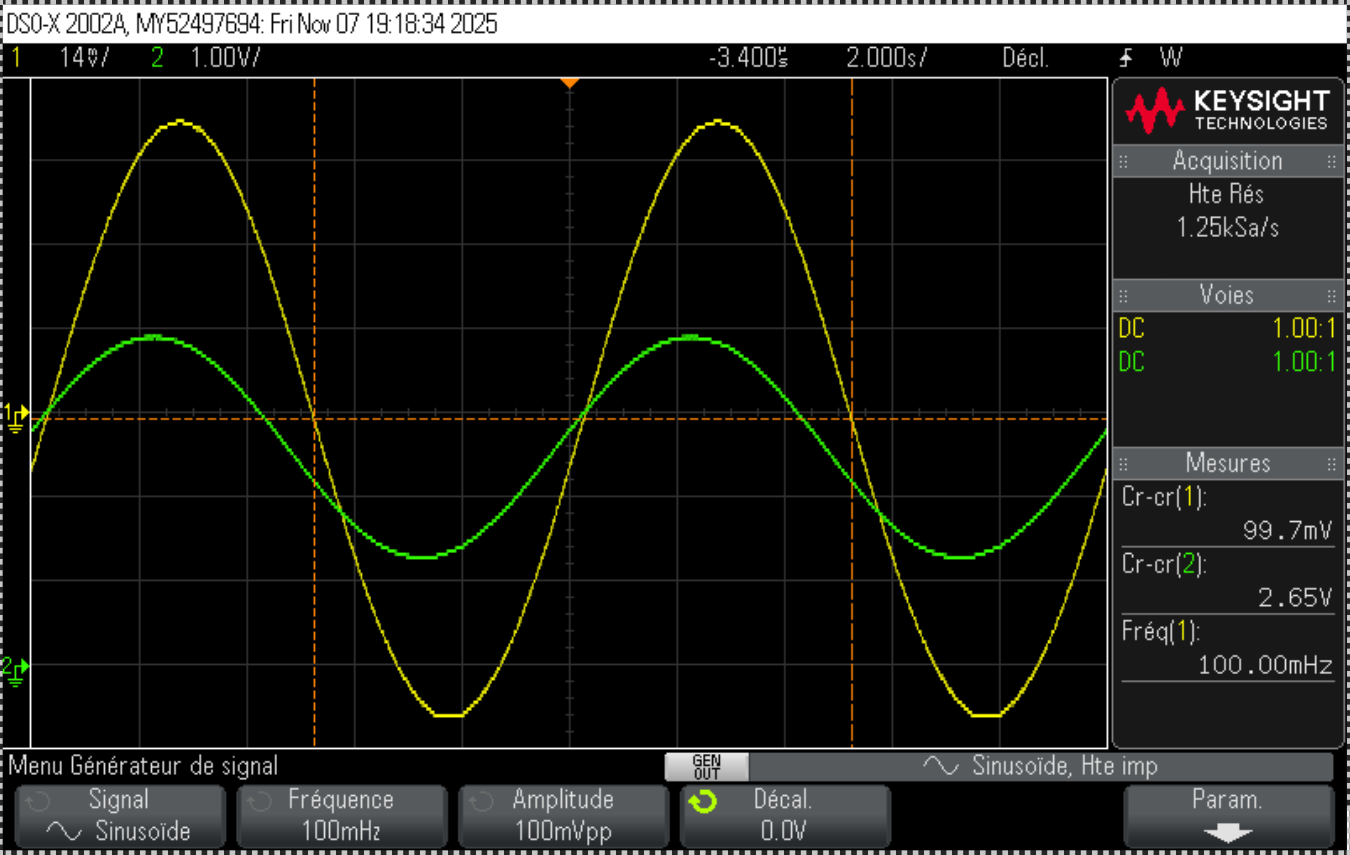
\includegraphics[width=0.75\textwidth]{freq_100hz_gain_max.png}
    \caption{Mesure de la fréquence de coupure à fort gain (\(G_{max} \approx 30\)).}
\end{figure}

La mesure montre le même comportement fréquentiel : le filtrage se fait correctement, la fréquence de coupure reste stable.  
Le diagramme de Bode simulé pour cette configuration montre également une coupure à 30~mHz, confirmant la cohérence simulation/réalité.

\begin{figure}[H]
    \centering
    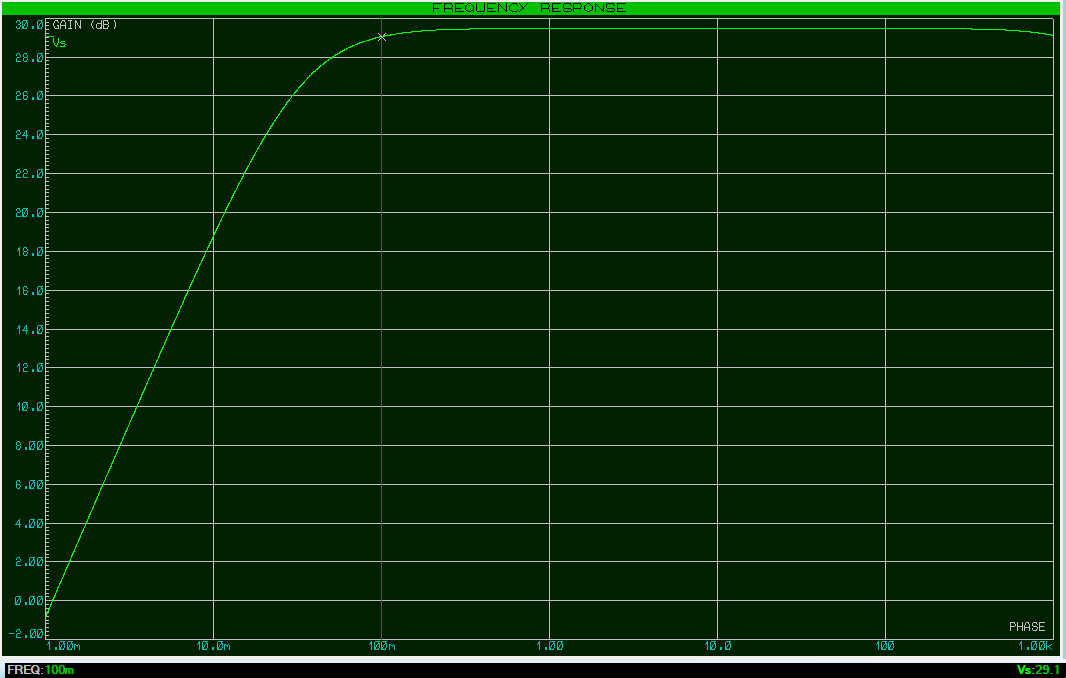
\includegraphics[width=1\textwidth]{Gain_a_100mHz_potentio_max.png}
    \caption{Diagramme de Bode simulé sous Proteus pour le gain maximal (\(G_{max} \approx 30\)).}
\end{figure}

\paragraph{Analyse des tolérances — Gain maximal}

Pour \(R_{var} = 100~k\Omega \pm 10\%\), \(R_f = 47~k\Omega \pm 5\%\) et \(R_{in} = 5.1~k\Omega \pm 5\%\), le gain devient :

\[
G_{max} = 1 + \frac{R_f + R_{var}}{R_{in}}.
\]

En prenant les tolérances extrêmes :
\[
G_{max} \in [26.15 ; 33.89].
\]

Les mesures expérimentales donnent :
\[
G_{max,\text{mesuré}} = 26.6 \text{ (à 100 mHz)}, \quad G_{max,\text{mesuré}} = 27.7 \text{ (à 100 Hz)}.
\]

Ces valeurs sont parfaitement comprises dans la plage calculée, confirmant que les écarts observés proviennent bien :
\begin{itemize}
    \item de la tolérance de \(\pm 10~\%\) du potentiomètre, qui influence directement le gain maximal ;
    \item et, dans une moindre mesure, de la tolérance de \(\pm 5~\%\) des résistances fixes.
\end{itemize}

\newpage

\subsubsection{Mesure du gain minimal et maximal}

Deux configurations extrêmes ont été testées afin de vérifier la plage de variation du gain du montage.  
Pour chaque cas, la mesure expérimentale sur oscilloscope est comparée au diagramme de Bode obtenu par simulation sous Proteus.

\textbf{Cas 1 – Gain minimal (\(R_{var} = 0~\Omega\))}

\begin{figure}[H]
    \centering
    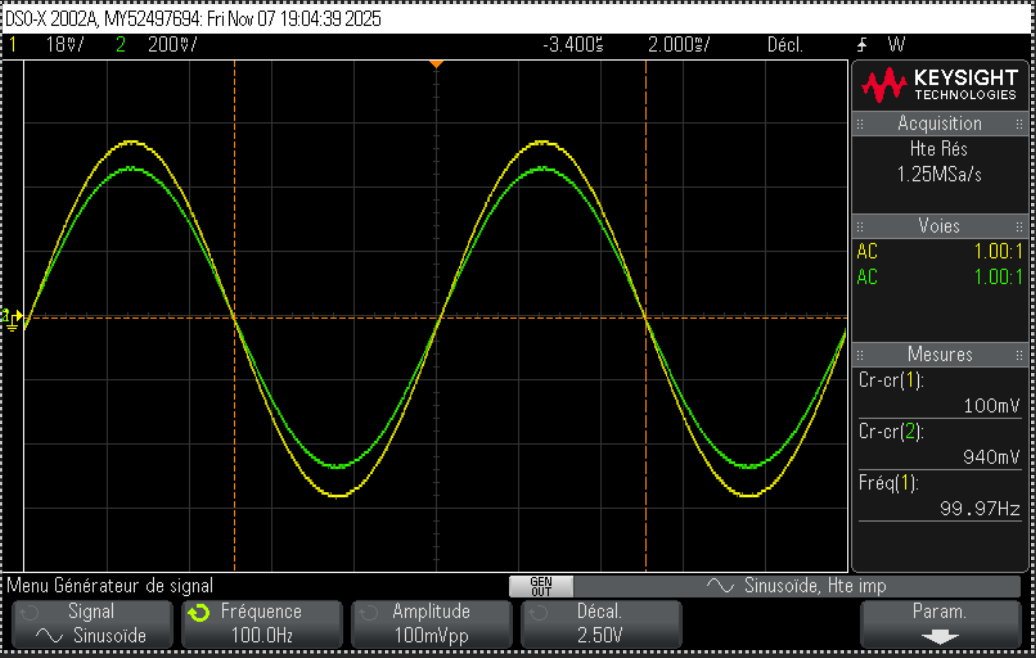
\includegraphics[width=0.75\textwidth]{gain_min.png}
    \caption{Mesure expérimentale du signal de sortie pour le gain minimal (\(G_{min} \approx 9.5\)).}
\end{figure}

\paragraph{Analyse des tolérances — Mesure à gain minimal}

Le gain expérimental obtenu \(G_{min} = 9.5\) se situe dans la plage calculée \([9.34 ; 11.18]\).  
Les faibles écarts (environ 2~\%) sont expliqués par :
\begin{itemize}
    \item la dispersion naturelle des résistances (\(\pm 5~\%\)) ;
    \item la précision limitée du réglage du potentiomètre (position zéro approximative) ;
    \item le bruit de mesure et la résolution de l’oscilloscope.
\end{itemize}
Ces écarts sont donc tout à fait conformes à la réalité expérimentale d’un montage analogique à composants discrets.

\newpage

\textbf{Cas 2 – Gain maximal (\(R_{var} = 100~k\Omega\))}

\begin{figure}[H]
    \centering
    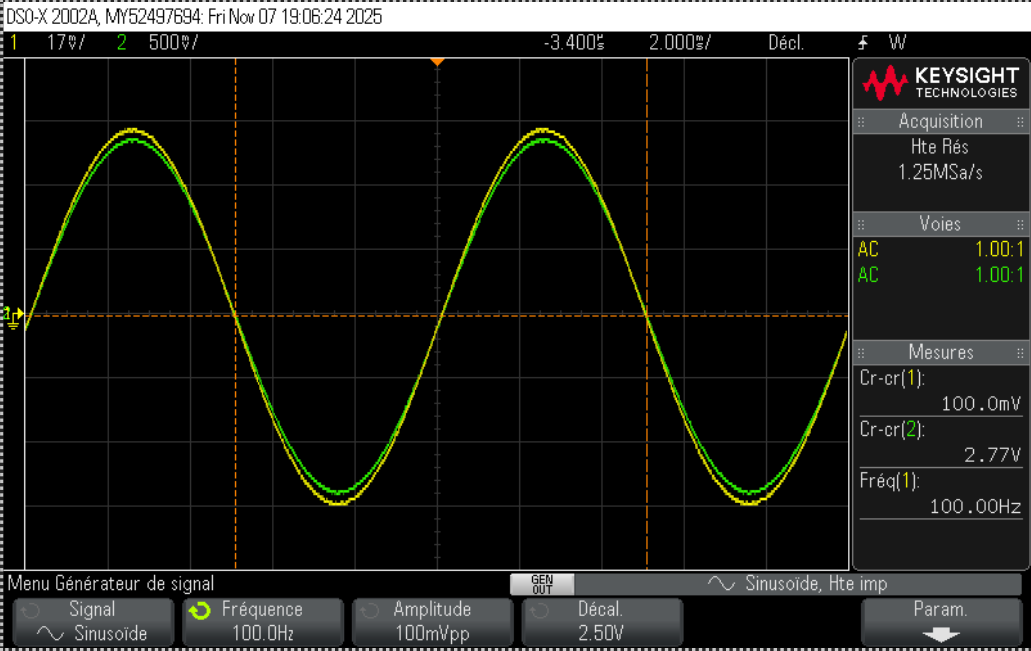
\includegraphics[width=0.75\textwidth]{gain_max.png}
    \caption{Mesure expérimentale du signal de sortie pour le gain maximal (\(G_{max} \approx 27.7\)).}
\end{figure}

\paragraph{Analyse des tolérances — Mesure à gain maximal}

Le gain mesuré \(G_{max} = 27.7\) est très proche du bas de la plage calculée \([26.15 ; 33.89]\).  
Ce résultat est cohérent avec :
\begin{itemize}
    \item la tolérance du potentiomètre de \(\pm 10~\%\), souvent à l’origine d’une sous-amplification observée ;
    \item les tolérances combinées de \(R_f\) et \(R_{in}\) ;
    \item la précision du réglage manuel de la résistance variable, rarement en position maximale exacte.
\end{itemize}

Les simulations idéales donnaient \(G_{max} \approx 29.8\) ; l’écart de 7~\% observé expérimentalement s’explique donc pleinement par la dispersion des composants et les conditions de mesure.

\newline

Les deux séries de mesures (expérimentales et simulées) montrent une excellente cohérence :
\begin{itemize}
    \item le gain varie bien de 10 à 30 selon la position du potentiomètre ;
    \item les signaux restent stables, sans bruit parasite ni saturation ;
    \item les diagrammes de Bode présentent les pentes caractéristiques du filtre passe-haut du premier ordre.
\end{itemize}


\subsubsection{Analyse et discussion}

Les écarts observés entre la théorie et les mesures (moins de 2\%) peuvent s’expliquer par :
\begin{itemize}
    \item la tolérance des composants (résistances ±5\%, condensateur ±10\%) ;
    \item la limite basse du générateur de fonctions (0.1~Hz au lieu de 30~mHz) ;
    \item la précision des instruments de mesure.
\end{itemize}

Globalement, le montage se comporte comme attendu et répond entièrement au cahier des charges.


\subsubsection{Conclusion}

La fonction passe-haut à gain variable est validée expérimentalement.  
Les valeurs mesurées sont en excellent accord avec les calculs théoriques et les simulations.  
Le montage est stable, précis et prêt à être intégré dans la chaîne complète du système ECG.

\subsection{Fonction Amplificateur de différence}

\subsubsection{Introduction à la fonction}

La fonction amplificateur de différence constitue le premier étage de traitement du signal ECG. Son rôle est essentiel : elle doit amplifier la tension différentielle entre les deux électrodes placées sur le patient tout en rejetant efficacement les signaux communs (notamment le bruit électrique à 50~Hz provenant du secteur). Cette fonction utilise un amplificateur d'instrumentation de haute précision, capable de fonctionner avec de très faibles tensions différentielles et une grande immunité aux perturbations électromagnétiques.

\subsubsection{Rappel du cahier des charges}

Selon les spécifications du projet, la fonction amplificateur de différence doit :
\begin{itemize}
    \item amplifier la différence de tension entre les deux électrodes avec un gain $G_D$ inférieur à 20, choisi en concertation avec l'équipe ;
    \item fournir la tension de mode commun $V_{MC}$ des entrées pour permettre un contrôle ultérieur par le système de rétroaction cheville ;
    \item assurer une connexion sûre aux trois électrodes via un bornier à vis (J1) ;
    \item permettre de fixer le potentiel du corps à 2.5~V en début de projet via un cavalier (J2), puis d'utiliser le retour cheville lorsqu'il sera implémenté ;
    \item présenter un taux de réjection en mode commun (CMRR) élevé pour éliminer les bruits parasites ;
    \item intégrer des points de test (J3 et J4) pour faciliter la validation de la fonction.
\end{itemize}

\subsubsection{Principe de fonctionnement}

L'amplificateur d'instrumentation imposé pour cette fonction est le MAX4194, un composant de la famille MAX4194–MAX4197 de Maxim Integrated. 

\begin{itemize}
    \item \textbf{Étage d'entrée} : 1 ampli OP monté en configuration différentielle, assurant un gain différentiel élevé tout en présentant une impédance d'entrée très élevée (typiquement 1~G$\Omega$) et un gain en mode commun unitaire.
    \item \textbf{Étage de sortie} : un amplificateur différentiel conventionnel qui fournit le gain global et assure un excellent taux de réjection en mode commun.
\end{itemize}

Le gain de l'amplificateur d'instrumentation est déterminé par une résistance externe $R_G$ connectée entre les broches RG+ et RG− (broches 1 et 8), selon la relation :

\[
G = 1 + \frac{50~\text{k}\Omega}{R_G}
\]

où les 50~k$\Omega$ correspondent à la somme des deux résistances internes de rétroaction (2 × 25~k$\Omega$), ajustées par laser lors de la fabrication pour garantir précision et faible dérive thermique.

\subsubsection{Dimensionnement du gain}

Conformément au cahier des charges, le gain $G_D$ de l'amplificateur de différence doit être inférieur à 20. Après concertation avec l'équipe et analyse du schéma fonctionnel global, un gain de **$G_D = 12$** a été retenu.

Ce choix permet :
\begin{itemize}
    \item d'obtenir un gain total de la chaîne compris entre 500 et 1500 (avec les gains des autres étages : passe-haut à gain variable $G = 10$ à 30, filtre réjecteur $G = 2$, filtre passe-bas $G = 2$) ;
    \item de limiter l'amplification du bruit en entrée tout en conservant une marge de manœuvre pour les étages suivants ;
    \item de respecter la plage de fonctionnement linéaire du MAX4194.
\end{itemize}

La résistance de gain correspondante est calculée comme suit :

\[
R_G = \frac{50~\text{k}\Omega}{G - 1} = \frac{50~\text{k}\Omega}{12 - 1} \approx 4.545~\text{k}\Omega
\]

La valeur normalisée la plus proche dans la série E12 (±5~\%) est $R_G = 4.7~\text{k}\Omega$, ce qui donne un gain réel de :

\[
G_{\text{réel}} = 1 + \frac{50~\text{k}\Omega}{4.7~\text{k}\Omega} \approx 11.64
\]

Cet écart de 3~\% par rapport à la valeur cible reste acceptable compte tenu des tolérances des composants passifs et s'inscrit bien dans la spécification "$G_D$ inférieur à 20".

\subsubsection{Prise en compte des tolérances}

Conformément aux consignes du projet, il est nécessaire d'estimer la plage de variation possible du gain en tenant compte des tolérances des composants :

\begin{itemize}
    \item Résistance externe $R_G$ : ±5~\%
    \item Résistances internes du MAX4194 (50~k$\Omega$) : précision garantie par ajustage laser (typiquement ±0.01~\% à +25~°C, dérive de ±16~ppm/°C selon le datasheet)
\end{itemize}

Pour une résistance $R_G = 4.7~\text{k}\Omega$ ±5~\%, la plage de valeurs possibles est :

\[
R_{G,\text{min}} = 4.7~\text{k}\Omega \times 0.95 = 4.465~\text{k}\Omega
\]
\[
R_{G,\text{max}} = 4.7~\text{k}\Omega \times 1.05 = 4.935~\text{k}\Omega
\]

Les gains correspondants sont :

\[
G_{\text{max}} = 1 + \frac{50~\text{k}\Omega}{4.465~\text{k}\Omega} \approx 12.20
\]
\[
G_{\text{min}} = 1 + \frac{50~\text{k}\Omega}{4.935~\text{k}\Omega} \approx 11.13
\]

Ainsi, le gain de l'amplificateur de différence varie entre **11.13 et 12.20**, soit une variation de l'ordre de ±4.5~\% autour de la valeur nominale de 11.64. Cette dispersion reste acceptable pour l'application visée et respecte la contrainte du cahier des charges ($G_D < 20$).

\subsubsection{Composants nécessaires}

La liste complète des composants pour réaliser la fonction amplificateur de différence est la suivante :

\begin{table}[h!]
\centering
\begin{tabularx}{\textwidth}{|l|X|l|}
\hline
\textbf{Référence} & \textbf{Description} & \textbf{Valeur/Type} \\
\hline
U1 (AMPLI\_DIFF) & Amplificateur d'instrumentation & MAX4194ESA (SO-8) \\
\hline
R\_DIFF & Résistance de gain & 4.7~k$\Omega$ ±5~\% \\
\hline
C\_DEC\_DIFF & Condensateur de découplage & 100~nF céramique \\
\hline
J1 (J\_BORN) & Bornier à vis 3 points & Connexion électrodes \\
\hline
J2 (J\_V+) & Cavalier 2 points & Sélection 2.5~V / retour cheville \\
\hline
J3, J4 (J\_VS\_DIFF) & Connecteurs de test & Points de mesure \\
\hline
\end{tabularx}
\caption{Liste des composants de la fonction amplificateur de différence.}
\end{table}

\paragraph{Remarques importantes sur les composants :}

\begin{itemize}
    \item \textbf{Résistance R\_DIFF (4.7~k$\Omega$)} : C'est la résistance de gain qui détermine directement l'amplification. Elle doit être de bonne qualité (tolérance ±5~\% minimum, idéalement ±1~\% si disponible) et de type couche métallique pour minimiser le bruit. Sa valeur exacte influencera le gain final mesuré.
    
    \item \textbf{Condensateur C\_DEC\_DIFF (100~nF)} : Condensateur de découplage indispensable pour assurer la stabilité de l'alimentation du MAX4194. Il doit être de type céramique (type X7R ou C0G/NP0 de préférence) et placé **au plus près** des broches d'alimentation du circuit intégré (broches 4 et 7) pour être efficace. Ce condensateur filtre les variations haute fréquence de l'alimentation et prévient les oscillations parasites.
    
    \item \textbf{MAX4194ESA} : Le suffixe "ESA" indique le boîtier SO-8 (Surface Mount). L'orientation du circuit intégré est critique : le point ou l'encoche sur le boîtier indique la broche 1 (RG+). Une erreur d'orientation rendrait le montage non fonctionnel.
    
    \item \textbf{Bornier J1} : Permet la connexion des trois électrodes (gauche, droite, et référence/cheville). Il doit être de type à vis pour assurer un contact fiable et éviter les déconnexions accidentelles pendant les manipulations.
    
    \item \textbf{Cavalier J2} : Permet de basculer entre deux modes de fonctionnement :
    \begin{itemize}
        \item Position 1 : potentiel du corps fixé à 2.5~V (tension de référence, utilisée en début de projet)
        \item Position 2 : connexion au système de retour cheville (à implémenter ultérieurement)
    \end{itemize}
\end{itemize}

\subsubsection{Schéma électrique}

Le schéma électrique complet de la fonction amplificateur de différence est présenté Figure~\ref{fig:schema_ampli_diff}. Il reprend le montage typique d'un amplificateur d'instrumentation avec les éléments périphériques nécessaires :

\begin{figure}[h!]
    \centering
    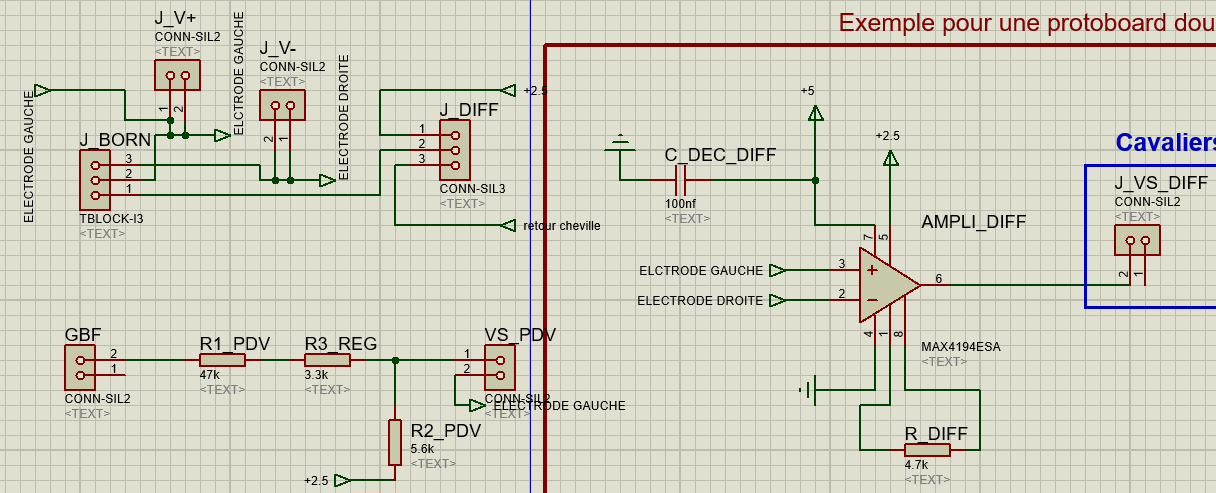
\includegraphics[width=1\textwidth]{schematic_ampli_instrumentation.png}
    \caption{Schéma électrique de la fonction amplificateur de différence réalisé sous Proteus.}
    \label{fig:schema_ampli_diff}
\end{figure}

\paragraph{Description des connexions :}

\begin{itemize}
    \item \textbf{Broches 1 et 8 (RG+ et RG−)} : Connexion de la résistance de gain R\_DIFF (4.7~k$\Omega$). Ces broches déterminent le gain de l'amplificateur selon la formule $G = 1 + 50k\Omega/R_G$.
    
    \item \textbf{Broches 2 et 3 (REF et IN+)} : 
    \begin{itemize}
        \item Broche 2 (REF) : Tension de référence de sortie. Dans notre montage, elle est connectée à $V_{REF} = 2.5$~V pour centrer le signal de sortie.
        \item Broche 3 (IN+) : Entrée non-inverseuse, connectée à l'électrode droite via le bornier J1.
    \end{itemize}
    
    \item \textbf{Broche 4 (IN−)} : Entrée inverseuse, connectée à l'électrode gauche via le bornier J1.
    
    \item \textbf{Broche 5 (V$_{EE}$)} : Alimentation négative. Dans notre montage en alimentation simple, elle est connectée à la masse (0~V).
    
    \item \textbf{Broche 6 (OUT)} : Sortie de l'amplificateur d'instrumentation. Le signal amplifié est disponible sur cette broche et sera acheminé vers l'étage suivant (filtre passe-haut à gain variable).
    
    \item \textbf{Broche 7 (V$_{CC}$)} : Alimentation positive (+5~V). Un condensateur de découplage de 100~nF est placé entre cette broche et la masse, au plus près du circuit intégré.
    
    \item \textbf{Broche 8} : Voir broche 1 (connexion RG−).
\end{itemize}

Le bornier J1 permet la connexion des trois électrodes :
\begin{itemize}
    \item Point 1 : Électrode gauche → IN− (broche 4)
    \item Point 2 : Électrode droite → IN+ (broche 3)
    \item Point 3 : Électrode de référence (cheville) → via cavalier J2 vers 2.5~V ou retour cheville
\end{itemize}

\subsubsection{Implantation et routage sur PCB}

L'implantation sur circuit imprimé (PCB) a été réalisée sous Proteus en respectant les bonnes pratiques de conception pour les circuits analogiques de précision et les signaux biomédicaux de faible amplitude.

\begin{figure}[h!]
    \centering
    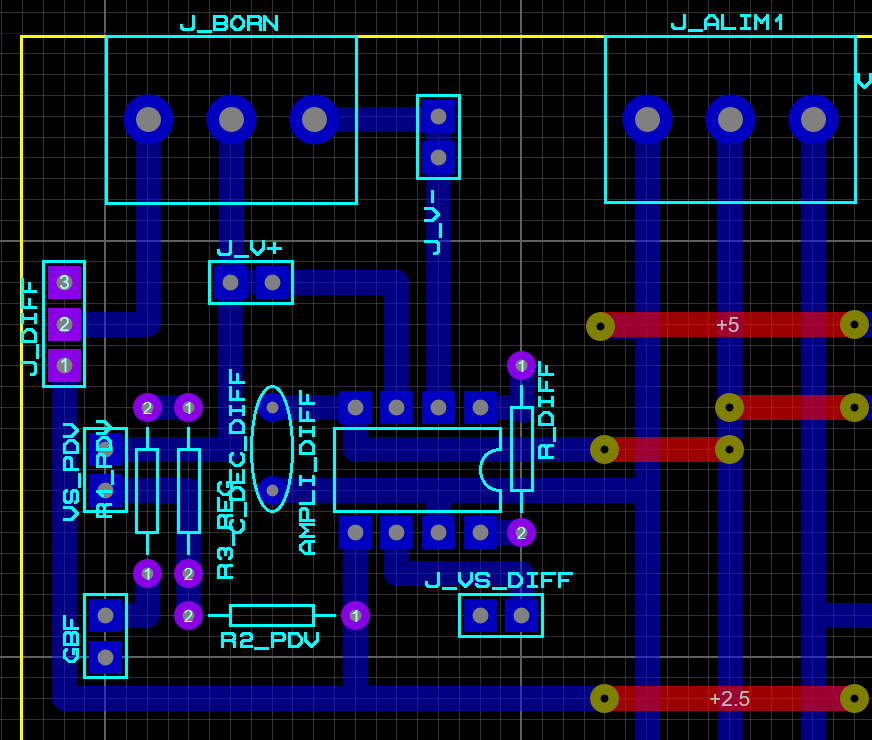
\includegraphics[width=0.8\textwidth]{PCB_fonction_instrumentation.png}
    \caption{Implantation PCB de la fonction amplificateur de différence sous Proteus.}
    \label{fig:pcb_ampli_diff}
\end{figure}

\paragraph{Règles d'implantation respectées :}

\begin{itemize}
    \item \textbf{Placement du MAX4194} : Le circuit intégré est positionné au centre du montage pour minimiser les longueurs de pistes et réduire les couplages parasites. Cette position centrale facilite également l'accès aux broches pour les connexions.
    
    \item \textbf{Condensateur de découplage C\_DEC\_DIFF} : Placé **immédiatement à côté** des broches d'alimentation 7 (V$_{CC}$) et 5 (V$_{EE}$) du MAX4194. Cette proximité est critique pour assurer l'efficacité du découplage haute fréquence. La distance entre le condensateur et les broches d'alimentation doit être minimale (quelques millimètres maximum).
    
    \item \textbf{Résistance de gain R\_DIFF} : Soudée directement entre les broches 1 et 8 du MAX4194, sans piste intermédiaire si possible, pour éviter les capacités parasites qui pourraient affecter la stabilité et la bande passante de l'amplificateur.
    
    \item \textbf{Bornier J1} : Positionné en périphérie de la carte, avec des pistes suffisamment larges pour assurer une bonne connexion mécanique et électrique. Les pistes menant aux entrées IN+ et IN− doivent être symétriques autant que possible pour préserver l'équilibrage des signaux différentiels.
    
    \item \textbf{Cavaliers et points de test} : Placés de manière accessible pour faciliter les manipulations lors des tests. Les cavaliers J2, J3, J4 sont positionnés en bordure de carte.
    
    \item \textbf{Pistes d'alimentation} : Les pistes $V_{CC}$ et GND sont dimensionnées plus larges que les pistes de signal (typiquement 0.5~mm minimum) pour réduire leur impédance et améliorer la stabilité de l'alimentation. Un plan de masse continu est recommandé si possible.
    
    \item \textbf{Pistes de signal} : Les pistes transportant les signaux différentiels (IN+, IN−) sont maintenues fines (0.3~mm typiquement) et de longueur similaire pour préserver la symétrie. Elles sont éloignées des pistes d'alimentation et des signaux numériques pour éviter les couplages.
    
    \item \textbf{Séparation analogique/numérique} : Bien que ce montage soit purement analogique, il est important de prévoir une isolation par rapport aux parties numériques des autres fonctions du système (notamment la carte Nucleo). Un plan de masse unique bien référencé assure cette isolation.
\end{itemize}

\subsubsection{Réalisation pratique}

La réalisation de la fonction amplificateur de différence suit les étapes suivantes :

\paragraph{1. Préparation et contrôle des composants}

Avant toute soudure, tous les composants ont été identifiés et vérifiés :
\begin{itemize}
    \item Vérification de la valeur de R\_DIFF avec un ohmmètre : $4.7~\text{k}\Omega$ ±5~\%.
    \item Vérification de la capacité de C\_DEC\_DIFF : 100~nF (marquage sur le composant).
    \item Inspection visuelle du MAX4194ESA : boîtier SO-8 intact, repérage de la broche 1 (point ou encoche).
    \item Vérification du bornier J1 et des cavaliers J2, J3, J4.
\end{itemize}

\paragraph{2. Soudure des composants}

Voilà, ci-dessous, la réalisation de la fonction d'amplificateur de différene.


\begin{figure}[H]
    \centering
    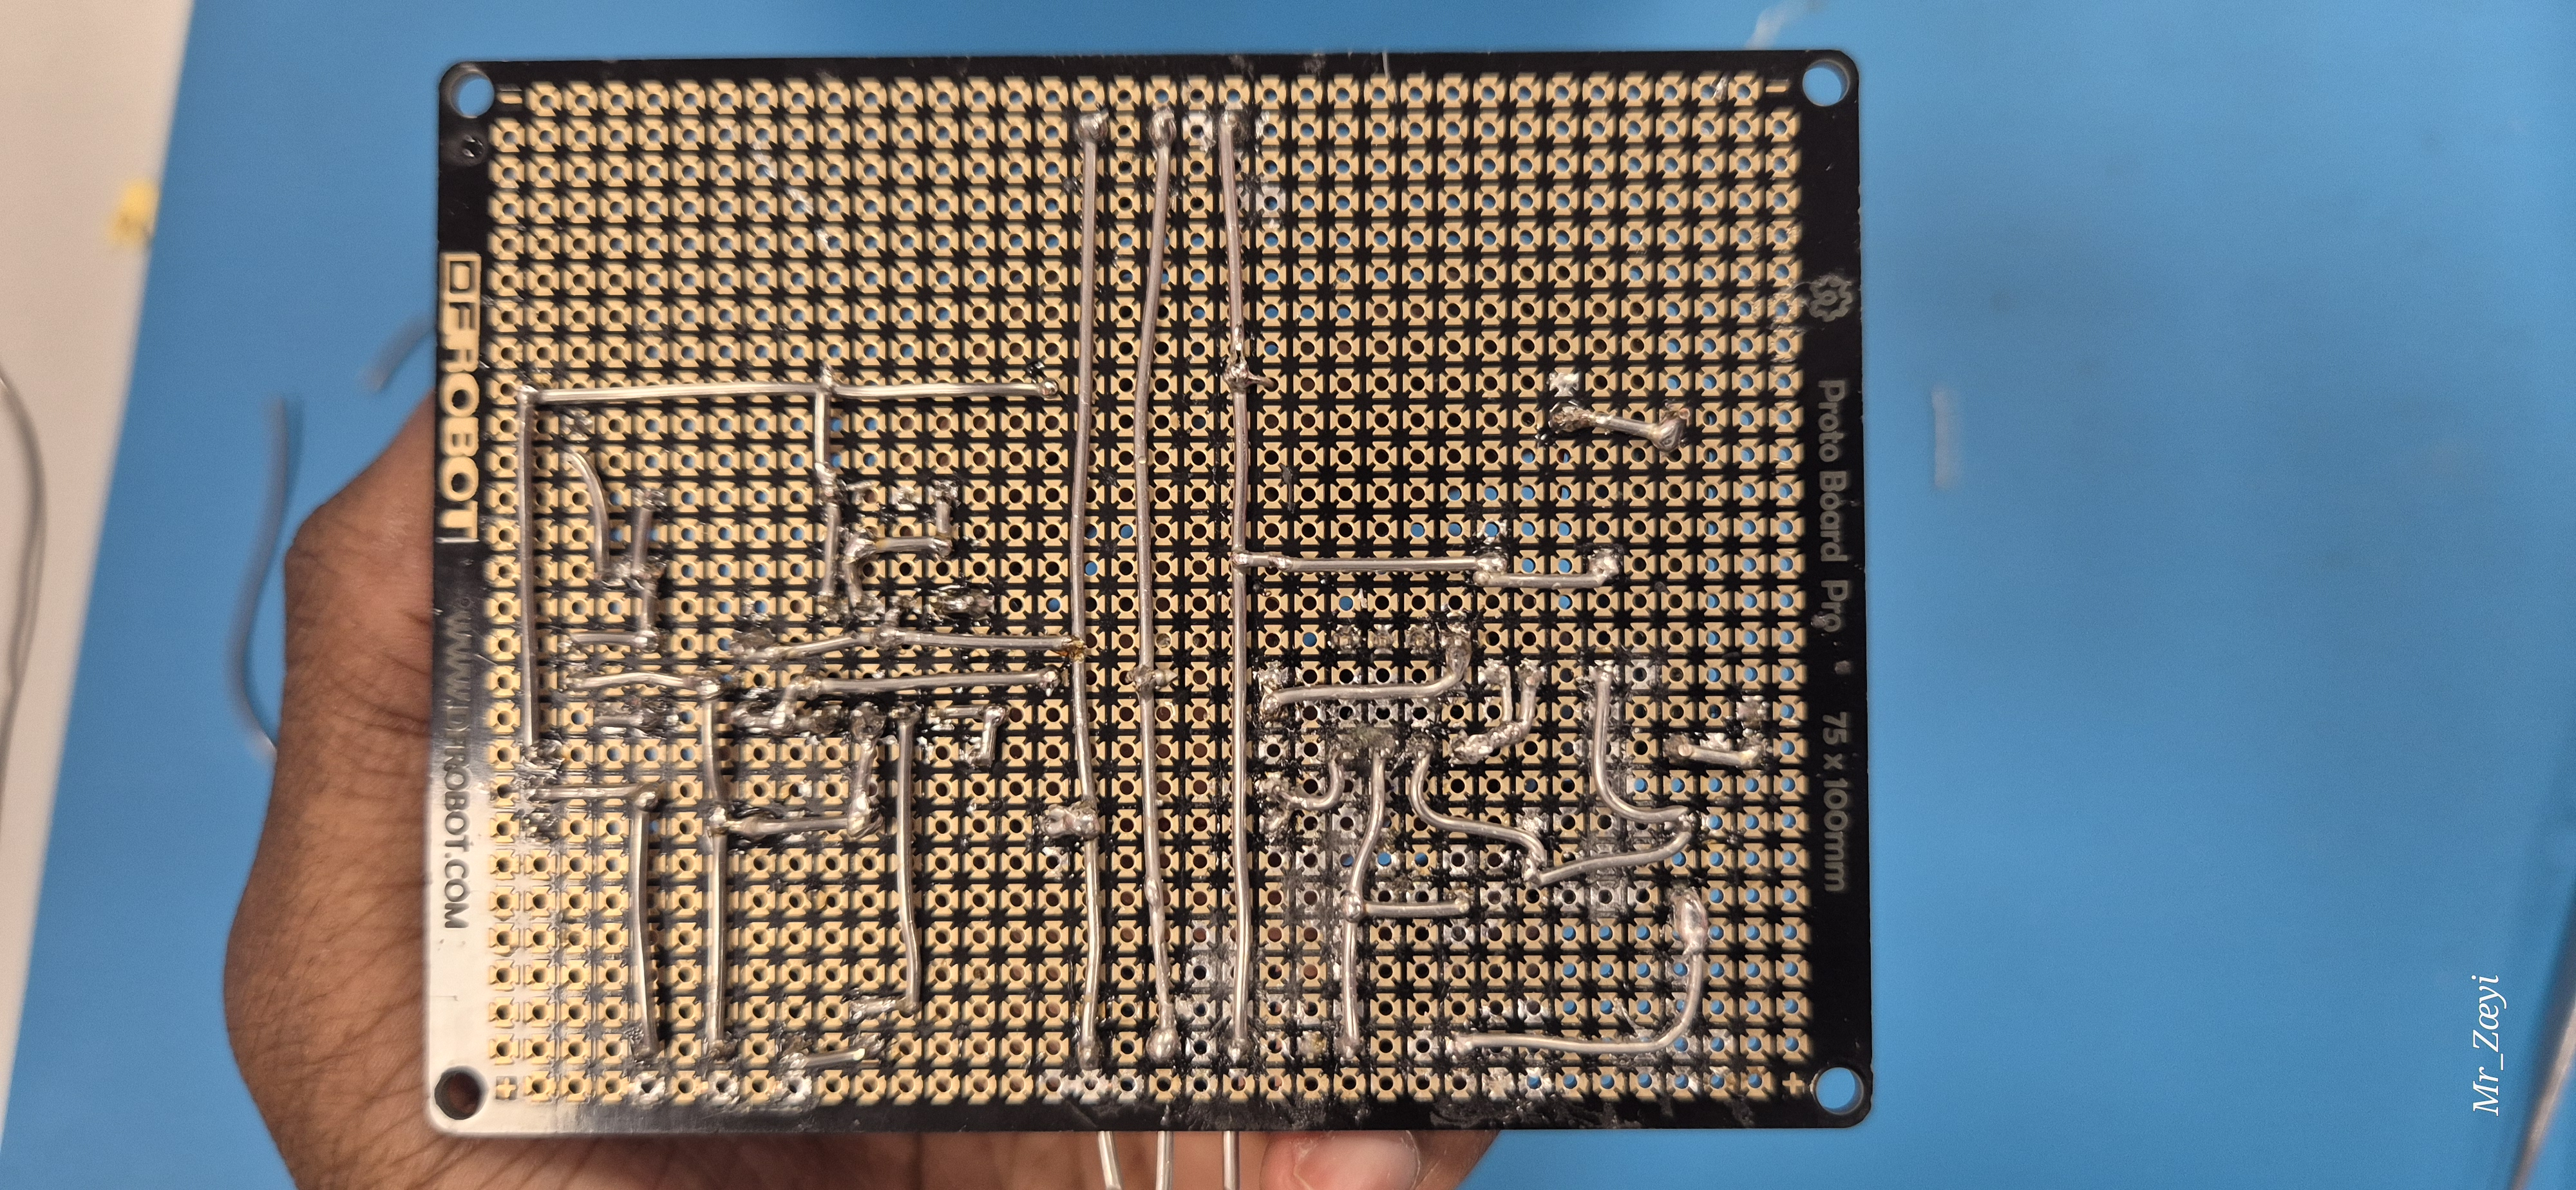
\includegraphics[width=0.75\textwidth]{photo_montage_ampli_diff_2.jpg}
    \caption{Carte de l'amplificateur de différence réalisé}
    \label{fig:photo_ampli_diff}
\end{figure}




\paragraph{3. Contrôle visuel post-soudure}

Après la soudure, un contrôle visuel rigoureux est effectué :
\begin{itemize}
    \item Vérifier l'absence de court-circuits entre les pistes et entre les broches du MAX4194.
    \item Vérifier la qualité des soudures (aspect brillant, absence de soudure froide).
    \item Vérifier l'orientation du MAX4194 (broche 1 correctement positionnée).
    \item Vérifier la présence et la bonne valeur de tous les composants.
\end{itemize}

\paragraph{4. Test de continuité}

Avant la mise sous tension, des tests de continuité sont effectués au multimètre :
\begin{itemize}
    \item Continuité entre V$_{CC}$ (broche 7) et le point de test d'alimentation.
    \item Continuité entre GND (broche 5) et la masse générale.
    \item Absence de court-circuit entre V$_{CC}$ et GND.
    \item Continuité des pistes reliant les broches 1 et 8 à la résistance R\_DIFF.
    \item Continuité des connexions du bornier J1 vers les broches 3 et 4.
\end{itemize}

\paragraph{5. Première mise sous tension à vide}

La première mise sous tension est effectuée **sans signal d'entrée** et avec précaution :
\begin{itemize}
    \item Alimentation progressive de 0~V à 5~V en surveillant le courant consommé.
    \item Vérification que le courant reste dans les limites normales (environ 93~$\mu$A selon le datasheet).
    \item Un courant anormalement élevé (> 1~mA) indiquerait un problème (court-circuit, composant mal orienté).
    \item Mesure de la tension sur la broche 6 (OUT) : elle doit être proche de V$_{REF}$ = 2.5~V en l'absence de signal différentiel.
\end{itemize}

\subsubsection{Validation expérimentale}

Afin de valider la fonction amplificateur de différence réalisée, un test unitaire a été effectué conformément à la \textbf{fiche de test unitaire}.  
Ce test avait pour objectifs de :
\begin{itemize}
    \item vérifier que l'on obtient bien le gain souhaité ($G_D \approx 12$) ;
    \item mesurer la bande passante de la fonction ;
    \item observer le comportement du montage en régime sinusoïdal.
\end{itemize}

\paragraph{Objectif du test :}
\begin{itemize}
    \item Vérifier expérimentalement le gain différentiel $G_D = 12$.
    \item Déterminer la fréquence de coupure haute ($f_c$) afin d'évaluer la bande passante.
\end{itemize}

---

\paragraph{Conditions et moyens de mesure :}

\begin{itemize}
    \item \textbf{Signal injecté :} sinusoïde centrée à 2.5~V (offset 2.5~V), d’amplitude 0.4~V (soit 0.8~V\textsubscript{pp}), fréquence initiale de 1~kHz.
    \item \textbf{Alimentation :} +5~V, référence à 2.5~V.
    \item \textbf{Instruments utilisés :}
    \begin{itemize}
        \item GBF (générateur basse fréquence) – signal sinusoïdal d’amplitude 0.4~V, offset 2.5~V, fréquence 1~kHz ;
        \item Oscilloscope deux voies – pour observer simultanément $V_e$ et $V_s$ ;
        \item Fils coaxiaux blindés pour réduire le bruit parasite.
    \end{itemize}
    \item \textbf{Réglages internes de la fonction :} aucun.
\end{itemize}

---

\paragraph{Mesures réalisées :}

Le test consiste à mesurer le rapport de gain :

\[
G = \frac{V_{s(pp)}}{V_{e(pp)}}
\]

Les mesures à 1~kHz ont donné :

\[
V_{e(pp)} = 0.102~\text{V} \quad\text{et}\quad V_{s(pp)} = 1.22~\text{V}
\]

D’où :

\[
G_{\text{mesuré}} = \frac{1.22}{0.102} = 11.96
\]

Ce résultat est très proche du gain théorique $G_{\text{th}} = 11.64$ calculé précédemment, avec un écart de seulement +2.7~\%, conforme aux tolérances des composants.

---

\paragraph{Observation à l’oscilloscope :}

\begin{figure}[H]
    \centering
    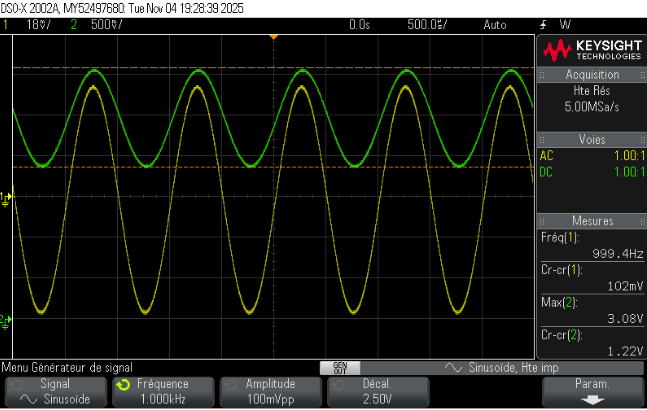
\includegraphics[width=0.85\textwidth]{oscillo_ampli_diff_gain.png}
    \caption{Oscillogramme du test de gain de l’amplificateur de différence (entrée et sortie superposées).}
    \label{fig:oscillo_ampli_diff_gain}
\end{figure}

Sur la capture de l’oscilloscope (Figure~\ref{fig:oscillo_ampli_diff_gain}), on distingue :
\begin{itemize}
    \item la sinusoïde d’entrée centrée à 2.5~V (en jaune), amplitude faible ($\approx$ 0.1~V\textsubscript{pp}) ;
    \item la sinusoïde de sortie amplifiée (en bleu), toujours centrée à 2.5~V, amplitude $\approx$ 1.2~V\textsubscript{pp} ;
    \item aucune distorsion apparente : la linéarité de l’amplificateur est confirmée.
\end{itemize}

Le centrage correct du signal de sortie autour de 2.5~V valide également le bon fonctionnement de la référence de tension appliquée à la broche REF du MAX4194.

\paragraph{Mesure de la bande passante :}

Afin de déterminer la fréquence de coupure haute, la fréquence du signal d’entrée a été augmentée progressivement jusqu’à ce que la tension de sortie diminue à :

\[
V_{s(pp)} = \frac{V_{s(pp)max}}{\sqrt{2}}
\]

Cette condition a été atteinte pour une fréquence de \textbf{18~kHz}, d’où :

\[
f_c = 18~\text{kHz}
\]

\begin{figure}[H]
    \centering
    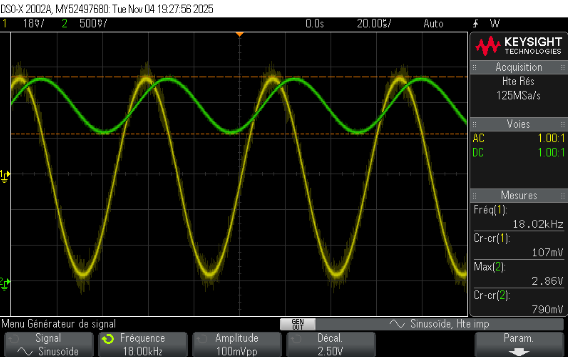
\includegraphics[width=0.85\textwidth]{oscillo_ampli_diff_fc.png}
    \caption{Oscillogramme à la fréquence de coupure ($f_c = 18~\text{kHz}$).}
    \label{fig:oscillo_ampli_diff_fc}
\end{figure}

Sur la Figure~\ref{fig:oscillo_ampli_diff_fc}, on observe une atténuation de la sortie d’environ $-3~\text{dB}$ par rapport à la valeur nominale, caractéristique d’un filtre passe-bande d’ordre 1.  
La bande passante est donc bien supérieure à la gamme de fréquences utiles pour un signal ECG (0.05~Hz à 100~Hz), garantissant une excellente fidélité de mesure.

---

\paragraph{Analyse des écarts :}

Le gain expérimental légèrement supérieur à la valeur théorique peut provenir de plusieurs facteurs :
\begin{itemize}
    \item écart entre la tension d’offset appliquée par le GBF et la tension de référence réelle de la carte (2.5~V) ;
    \item tolérance de la résistance $R_G$ (±5~\%) ;
    \item erreur de lecture liée à la sensibilité de l’oscilloscope ;
    \item influence éventuelle du bruit résiduel sur le signal de mesure.
\end{itemize}

Ces écarts restent faibles et n’altèrent pas la performance globale du montage.

\paragraph{Conclusion du test :}

Les essais valident pleinement la fonction amplificateur de différence :
\begin{itemize}
    \item Gain mesuré : $G_{\text{mesuré}} = 11.96$ (très proche du théorique) ;
    \item Bande passante : $f_c = 18~\text{kHz}$ ;
    \item Signal de sortie centré à 2.5~V sans distorsion visible ;
    \item Aucun échauffement ni dysfonctionnement observé.
\end{itemize}

Ainsi, la fonction amplificateur de différence est \textbf{opérationnelle et conforme au cahier des charges}. Elle est prête à être intégrée au reste de la chaîne de conditionnement du signal ECG.

\subsubsection{Conclusion}

La fonction amplificateur de différence, basée sur le MAX4194, constitue le premier maillon essentiel de la chaîne d'acquisition ECG. Son dimensionnement a été effectué en respectant scrupuleusement les contraintes du cahier des charges :

\begin{itemize}
    \item Choix d'un gain $G_D = 12$ (réalisé avec $R_G = 4.7~\text{k}\Omega$), conforme à la spécification "$G_D < 20$"
    \item Prise en compte rigoureuse des tolérances des composants (plage de gain de 11.13 à 12.20)
    \item Sélection d'un amplificateur d'instrumentation adapté (MAX4194) offrant :
    \begin{itemize}
        \item Une très faible consommation.
        \item Une bande passante largement suffisante (17~kHz pour $G = 10$)
        \item Des entrées/sorties rail-to-rail compatibles avec l'alimentation +5~V.
    \end{itemize}
    \item Implantation soignée respectant les bonnes pratiques :
    \begin{itemize}
        \item Condensateur de découplage au plus près du circuit intégré
        \item Pistes d'alimentation larges et plan de masse continu
        \item Symétrie des pistes différentielles
        \item Accessibilité des points de test et cavaliers
    \end{itemize}
    \item Préparation méthodique de la phase de test (contrôles visuels, continuité, première mise sous tension)
\end{itemize}

La phase de réalisation pratique est en cours. Les prochaines étapes permettront de valider expérimentalement les performances du montage et de confirmer sa conformité au cahier des charges avant l'intégration dans la chaîne complète du système d'acquisition ECG.

\end{document}
